\documentclass[a4paper]{book}
\usepackage{amssymb}
\usepackage{amsmath}
\usepackage{multicol}
\usepackage{fancyhdr}
\usepackage{hyperref}
\usepackage{listings}
\usepackage{color}
\usepackage{tikz}
\usetikzlibrary{shapes,arrows}
\usepackage{pgfplots}
\usepackage{pgfplotstable}
\usepackage{graphicx}
\usepackage[]{mdframed}
\usepackage{algorithm2e}
\usepackage{svg}
\usepackage{enumitem}
\usepackage{refcount}
\usepackage{cleveref}
\usepackage{cite}
\usepackage{bookmark}
\usepackage{mathtools}


% draw a frame around given text
\newcommand{\coderef}[1]{%
  \hyperref[#1]{Code \numberstringnum{\getrefnumber{#1}}}%
}
\newcommand{\argmin}{\operatornamewithlimits{argmin}}
\newcommand{\framedtext}[1]{%
\vspace{1em}%
\par%
\noindent\fbox{%
    \parbox{\dimexpr\linewidth-2\fboxsep-2\fboxrule}{#1}%
}%
\vspace{1em}%
}
\SetKwComment{Comment}{\# }{}
\newcommand{\norm}[1]{\left\lVert#1\right\rVert}


% CUSTOM COMMANDS
\newcommand{\image}[1]{\begin{center}\includegraphics[width=.75\linewidth]{#1}\end{center}}

% reference to a figure incl. "Figure"
\newcommand{\figref}[1]{\figurename~\ref{#1}}
\newcommand{\tabref}[1]{\tablename~\ref{#1}}

% comment command

\newcommand{\comment}[1]{}

% Math

\newcommand{\K}{\mathbb{K}}
\newcommand{\G}{\mathbb{G}}
\newcommand{\N}{\mathbb{N}}
\newcommand{\R}{\mathbb{R}}
\newcommand{\MSE}{\text{MSE}}
\newcommand{\RMSE}{\text{RMSE}}
\newcommand{\MAE}{\text{MAE}}
\newcommand{\GIoU}{\text{GIoU}}
\newcommand{\IoU}{\text{IoU}}
\newcommand{\PCA}{\text{PCA}}
\newcommand*{\qed}{\null\nobreak\hfill\ensuremath{\blacksquare}}
\DeclareMathOperator{\e}{e}
\DeclareMathOperator{\Hyp}{Hyp}
\DeclareMathOperator{\Normal}{N}
\DeclareMathOperator{\Binomial}{B}
\DeclareMathOperator*{\argmin}{argmin}
\DeclareMathOperator*{\argmax}{argmax}
\DeclarePairedDelimiter\floor{\lfloor}{\rfloor}
\newcommand{\skr}[1]{\left\langle#1\right\rangle}
\newcommand{\norm}[1]{\left\lVert#1\right\rVert}

\newcommand{\mybold}[1]{\bm{#1}}
% Color definitions
\definecolor{YellowGreen}{RGB}{154, 205, 50}
\definecolor{BurntOrange}{RGB}{255, 165, 0}
\definecolor{CornflowerBlue}{RGB}{100, 149, 237}


% Code listing format for JSON file format
\colorlet{punct}{red!60!black}
\definecolor{background}{HTML}{EEEEEE}
\definecolor{delim}{RGB}{20,105,176}
\colorlet{numb}{magenta!60!black}

\lstdefinelanguage{json}{
    basicstyle=\normalfont\ttfamily,
    numbers=left,
    numberstyle=\scriptsize,
    stepnumber=1,
    numbersep=8pt,
    showstringspaces=false,
    breaklines=true,
    frame=lines,
    backgroundcolor=\color{background},
    literate=
     *{0}{{{\color{numb}0}}}{1}
      {1}{{{\color{numb}1}}}{1}
      {2}{{{\color{numb}2}}}{1}
      {3}{{{\color{numb}3}}}{1}
      {4}{{{\color{numb}4}}}{1}
      {5}{{{\color{numb}5}}}{1}
      {6}{{{\color{numb}6}}}{1}
      {7}{{{\color{numb}7}}}{1}
      {8}{{{\color{numb}8}}}{1}
      {9}{{{\color{numb}9}}}{1}
      {:}{{{\color{punct}{:}}}}{1}
      {,}{{{\color{punct}{,}}}}{1}
      {\{}{{{\color{delim}{\{}}}}{1}
      {\}}{{{\color{delim}{\}}}}}{1}
      {[}{{{\color{delim}{[}}}}{1}
      {]}{{{\color{delim}{]}}}}{1},
}

%% CNN + Tikz

\DeclareMathOperator{\ReLU}{ReLU}
\newcommand{\KL}{\ensuremath{\mathrm{KL}}}
\newcommand{\Ber}{\ensuremath{\mathrm{Ber}}}

\definecolor{fc}{HTML}{1E90FF}
\definecolor{h}{HTML}{228B22}
\definecolor{bias}{HTML}{87CEFA}
\definecolor{denseBlock}{HTML}{87CEFA}
\definecolor{noise}{HTML}{8B008B}
\definecolor{dropout}{HTML}{FFCCCB}
\definecolor{conv}{HTML}{FFA500}
\definecolor{dense}{HTML}{CDF3CD}
\definecolor{pool}{HTML}{FFD700}
\definecolor{up}{HTML}{B22222}
\definecolor{view}{HTML}{FFFFFF}
\definecolor{bn}{HTML}{FFD700}
\tikzset{fc/.style={black,draw=black,fill=fc,rectangle,minimum height=1cm}}
\tikzset{h/.style={black,draw=black,fill=h,rectangle,minimum height=1cm}}
\tikzset{bias/.style={black,draw=black,fill=bias,rectangle,minimum height=1cm}}
\tikzset{denseBlock/.style={black,draw=black,fill=denseBlock,rectangle,minimum height=1cm}}
\tikzset{noise/.style={black,draw=black,fill=noise,rectangle,minimum height=1cm}}
\tikzset{dropout/.style={black,draw=black,fill=dropout,rectangle,minimum height=1cm}}
\tikzset{conv/.style={black,draw=black,fill=conv,rectangle,minimum height=1cm}}
\tikzset{dense/.style={black,draw=black,fill=dense,rectangle,minimum height=1cm}}
\tikzset{pool/.style={black,draw=black,fill=pool,rectangle,minimum height=1cm}}
\tikzset{up/.style={black,draw=black,fill=up,rectangle,minimum height=1cm}}
\tikzset{view/.style={black,draw=black,fill=view,rectangle,minimum height=1cm}}
\tikzset{bn/.style={black,draw=black,fill=bn,rectangle,minimum height=1cm}}
\tikzset{basic/.style={draw,fill=blue!20,text width=1em,text badly centered}}
\tikzset{functions/.style={basic,circle,fill=blue!10}}




% HEADER/FOOTER DEFINITIONS

\newcommand{\pageHead}{[WIP] \leftmark}

\fancyhf{}
\lhead{\tiny\pageHead}
\rhead{\tiny\rightmark}
\rfoot{Page \thepage}
\lfoot{\author}

\definecolor{codegreen}{rgb}{0,0.6,0}
\definecolor{codegray}{rgb}{0.5,0.5,0.5}
\definecolor{codepurple}{rgb}{0.58,0,0.82}
\definecolor{backcolour}{rgb}{0.95,0.95,0.92}

\lstdefinestyle{mystyle}{
    backgroundcolor=\color{backcolour},   
    commentstyle=\color{codegray},
    keywordstyle=\color{blue},
    numberstyle=\tiny\color{white},
    stringstyle=\color{codegreen},
    basicstyle=\ttfamily\footnotesize,
    breakatwhitespace=false,         
    breaklines=true,                 
    captionpos=b,                    
    keepspaces=true,                 
    numbers=left,                    
    numbersep=5pt,                  
    showspaces=false,                
    showstringspaces=false,
    showtabs=false,                  
    tabsize=2
}

\lstset{style=mystyle}

\begin{document}
\pagestyle{fancy}
%\begin{multicols}{2}
\pagenumbering{Roman}% Capital 'R': uppercase Roman numerals
\chapter*{Preface}
\addcontentsline{toc}{chapter}{\protect\numberline{}Preface}
\label{ch:preface}

What is this book about?

What is the scope of this book?

Why is research in the field important?

Why is there a need for the information contained in this book?

\newpage
{
  % version and copyright
  \vspace*{\fill}
  \begin{center}
    \begin{minipage}{0.8\textwidth}
      \begin{center}
        \textbf{Version 0.0.0a}
      \end{center}
      \begin{flushright}
        \textbf{© 2023, \theauthor}\\
        \textbf{All rights reserved.}
      \end{flushright}
    \end{minipage}
  \end{center}
}

\newpage
\pagenumbering{arabic}% Capital 'R': uppercase Roman numerals
\tableofcontents
%\end{multicols}
\newpage

\setcounter{page}{1}
\chapter{Introduction}
\framedtext{\color{red}{TODO:}}



\chapter{Mathematics}
\label{ch:math}
The following chapter will give a brief introduction to the Mathematics required to get started in the realm of Data Science/Machine Learning.
There are many more things to cover, but this would go beyond of the scope of this book. The following chapter will only cover the most important concepts and provide links to further reading, as well as whenever possible, to implementations of the concepts. 
Apart from this further resources will provide for deeper research, whenever necessary.

The former is extremely important and will during the daily life as a Machine Learning Engineer or Data Scientist one will spend 80\% of the time 
\begin{itemize}
  \item Collecting Data
  \begin{itemize}
    \item Web Scraping
    \item searching for similar data sets
    \item Manual labelling of existing data
  \end{itemize}
  \item Preprocessing Data
  \begin{itemize}
    \item Data Cleaning
    \item Data Normalization
    \item Feature Engineering
    \item Exploring Data
    \item Visualizing Data
  \end{itemize}
\end{itemize}

The remaining 20\% will be spent on
\begin{itemize}
  \item Developing an ML Model
  \begin{itemize}
    \item Choosing the right Model
    \item Choosing the right Hyperparameters
    \item Training the Model
    \item Evaluating the Model
  \end{itemize}
\end{itemize}
Throughout all ML projects one will encounter a lot of Mathematics as well as Computer Science and must apply different techniques of linear algebra and probability theory.

Apart from this fundamental knowledge, one must also be able to read and understand scientific papers, which are usually written in a very formal and mathematical language. 

This document will list most required techniques and areas in Mathematics that are required to get started in the field of Machine Learning. It will not go into detail on how to implement these techniques, but rather give a brief overview of the most important concepts and provide links to further reading.

Before we get started, let's review some terms we will use in the following document.

\section{Vectors}
We're assuming that the reader has a general understanding of vectors.
Let $\vec{x} \in \R^n$ be a list of $n$ numbers, which can be written as a column or row. This is called a vector. 
The notation $\vec{x} \in \R^n$ represents a row-vector of $n$ real-valued numbers. $\vec{x} \in \R^{1 \times m}$ represents a column-vector of $1$ row and $m$ columns.
\subsection{Operators}
Vectors can be combined using basic arithmetic operators, such as addition, subtraction, multiplication and division.

\textbf{Addition} is defined as follows:
\begin{align*}
  f&(\vec{x}, \vec{y}) \rightarrow \vec{z},\\
  f&: (\R^n, \R^n) \mapsto \R^n\\
  &\vec{x} + \vec{y} = \begin{bmatrix}
    x_1 + y_1 \\ x_2 + y_2 \\ \vdots \\ x_n + y_n
  \end{bmatrix} = \vec{z}
\end{align*}\\
\textbf{Multiplication with a scalar (Scaling)} is defined as follows:
\begin{align*}
  f&(\vec{x}, \lambda) \rightarrow \vec{z},\\
  f&: (\R^n, \R) \mapsto \R^n\\
  &\vec{x} = \begin{bmatrix}
    \lambda x_1 \\ \lambda x_2 \\ \vdots \\ \lambda x_n
  \end{bmatrix} = \vec{z}
\end{align*}
Subtraction and Division are defined analogously.
Of course these operations can also be combined, e.g.:
\begin{align*}
  \lambda \vec{x} - \frac{1}{\beta} \vec{y} = \begin{bmatrix}
    \lambda x_1 - \frac{1}{\beta} y_1 \\ \lambda x_2 - \frac{1}{\beta} y_2 \\ \vdots \\ \lambda x_n - \frac{1}{\beta} y_n
  \end{bmatrix}
\end{align*}

Apart from the \dq Standard\dq operations, there are also some special operations that are defined on vectors. These are:
\begin{itemize}
  \item Dot Product
  \item Hadamard Product
\end{itemize}
and a few more. Here we will only look into the Dot Product and the Hadamard Product.

The \textbf{Dot Product}, or \textbf{Scalar Product}, is defined as follows:
\begin{align*}
  f&(\vec{x}, \vec{y}) \rightarrow \vec{z},\\
  f&: (\R^n, \R^n) \mapsto \R\\
  &\vec{x} \cdot \vec{y} = \sum_{i=1}^{n} x_i y_i = x_1 y_1 + x_2 y_2 + \dots + x_n y_n
\end{align*}
it can be used as a similarity measure between two vectors. The larger the dot product, the more similar the vectors are.

The \textbf{Hadamard Product}, the element-wise Product, is defined as follows:
\begin{align*}
  f&(\vec{x}, \vec{y}) \rightarrow \vec{z},\\
  f&: (\R^n, \R^n) \mapsto \R^n\\
  &\vec{x} \circ \vec{y} = \begin{bmatrix}
    x_1 y_1 \\ x_2 y_2 \\ \vdots \\ x_n y_n
  \end{bmatrix}
\end{align*}

Last, but not least, there is the operator of \textit{Transposition}. Transposition is defined as follows:
\begin{align*}
  f&(\vec{x}) \rightarrow \vec{z},\\
  f&: (\R^n) \mapsto \R^{1 \times n}\\
  &\vec{x}^T = \begin{bmatrix}
    x_1 & x_2 & \dots & x_n
  \end{bmatrix}
\end{align*}
This operator transforms a column-vector into a row-vector and vice versa.

\subsection{Norms}
In order to compare vectors another group of operators is required, the so called norms.
For vectors these are the $p$-norms, the $L^p$-norms and the $L^{\infty}$-norm.

The three most commonly used norms are the $L^1$-norm, the $L^2$-norm and the $L^{\infty}$-norm. The general $L^p$-norm is defined as follows:
\begin{align*}
  f&(\vec{x}) \rightarrow \vec{z},\\
  f&: (\R^n) \mapsto \R\\
  &\norm{\vec{x}}_p = \left(\sum_{i=1}^{n} \abs{x_i}^p\right)^{\frac{1}{p}}
  \end{align*}
The $L^1$-norm is also called the \textit{Manhattan Distance} or \textit{Taxicab Norm}. It has the following definition:
\begin{align*}
  f&(\vec{x}) \rightarrow \vec{z},\\
  f&: (\R^n) \mapsto \R\\
  &\norm{\vec{x}}_1 = \sum_{i=1}^{n} \abs{x_i}
\end{align*}
The $L^2$-norm is also called the \textit{Euclidean Norm}, the vector's length, and is defined as follows:
\begin{align*}
  f&(\vec{x}) \rightarrow \vec{z},\\
  f&: (\R^n) \mapsto \R\\
  &\norm{\vec{x}}_2 = \sqrt{\sum_{i=1}^{n} \abs{x_i}^2}
\end{align*}
And the $L^{\infty}$-norm is defined as:
\begin{align*}
  f&(\vec{x}) \rightarrow \vec{z},\\
  f&: (\R^n) \mapsto \R\\
  &\norm{\vec{x}}_{\infty} = \max_{i=1}^{n} \abs{x_i}
\end{align*}

Mainly the $L^1$-norm and the $L^2$-norm are used in Machine Learning. The $L^1$-norm is used when the number of features is very large and only a few of them are important. The $L^2$-norm is used when all features are important.
But we will see more about this throughout the document.

\textbf{Note:} The $L^2$-norm indicates the length of a vector and can be used to \textit{rescale} the vector to unit length.

Earlier we've mentioned the Dot-Product to be a measure of similarity, but this is not fully correct. We can only apply the Dot-Product as a similarity measure if we ensure that the vectors that are being compared have the same length. For this purpose we usually scale all vectors to unit length ($\frac{\vec{v}}{||\vec{v}||_2}$).

\section{Matrices}
Matrices are very closely related to vectors. A matrix is a two-dimensional array of numbers. A matrix can be written as a list of column-vectors or row-vectors. The notation $\mat{X} \in \R^{n \times m}$ represents a matrix of $n$ rows and $m$ columns. The notation $\mat{X} \in \R^{n \times 1}$ represents a column-vector of $n$ rows and $1$ column. The notation $\mat{X} \in \R^{1 \times m}$ represents a row-vector of $1$ row and $m$ columns.
\section{Derivatives}
\section{Probabilities}

\framedtext{\color{red}{TODO:}}



\chapter{Nearest Centroid Classifier}
\label{ch:ncc}
The first classification algorithm we will look into is the Nearest Centroid Classidfier.
It is a widely used algorithm for classification and is also one of the simplest ones to implement.
We will start by looking at the mathematical background of the algorithm and then implement it in Python.
This will help us to understand how to derive a classification algorithm from a mathematical model as well as the
limitations of machine learning models regarding assumptions it has towards the data.
Apart from this, the NNC is easy to interpret and easy to implement, which is a great starting point to get familiar with 
the Python programming language and the libraries we will use in this book.

\section{Motivation}
As in previous chapters mentioned, neuro scientists and other researchers used the brain as a blueprint for
designing theories. If we think about the neurology that is happening when
we want to do a categorization we understand on a neuronal level what happens to our brain.
Of course, only to some extend for some classes of cells. And we understand how humans
arrive at a certain category through psychological experiments. But we do not understand
how the brain is able to do this.
Between these two areas there is a huge gap. There is some research that tries to bridge this gap and ML could be a way to do this.
At last by providing some Prove of Concept (PoC) to those theories.
We will use a very simple psychological idea to explain the relation between the NCC and Linear Classifiers.
Linear Classification is on of the most frequently used techniques in Machine Learning. Even you do it, probably on a daily basis.
Now, we will bridge between the NCC and Linear Classifiers. But first we will try to understand the idea of classification through a psychological model.


\framedtext{
  \textbf{Imagine you are a Neuron.}

  You receive a non-linear filtered sensort input $\vec{x}$, e.g. a visual input from your eyes, a smell from your nose or a noice from your ears.

  \textit{How can we build abstract concepts from this information input?}

  In other words, \textit{how do humans categorize different stimuli?}
}\newline
For simplicity and to be able to visualize things we will imagine we only receive a 2 dimensional input.\\
First, we know all our data is $\vec{x} \in \mathbb{R}^2$. For example the bottom right triangle in Figure \ref{fig:prototypes_1} could be 
$\vec{x} = \begin{pmatrix}3\\2.5\end{pmatrix}$

\begin{figure}[h]
  \centering
  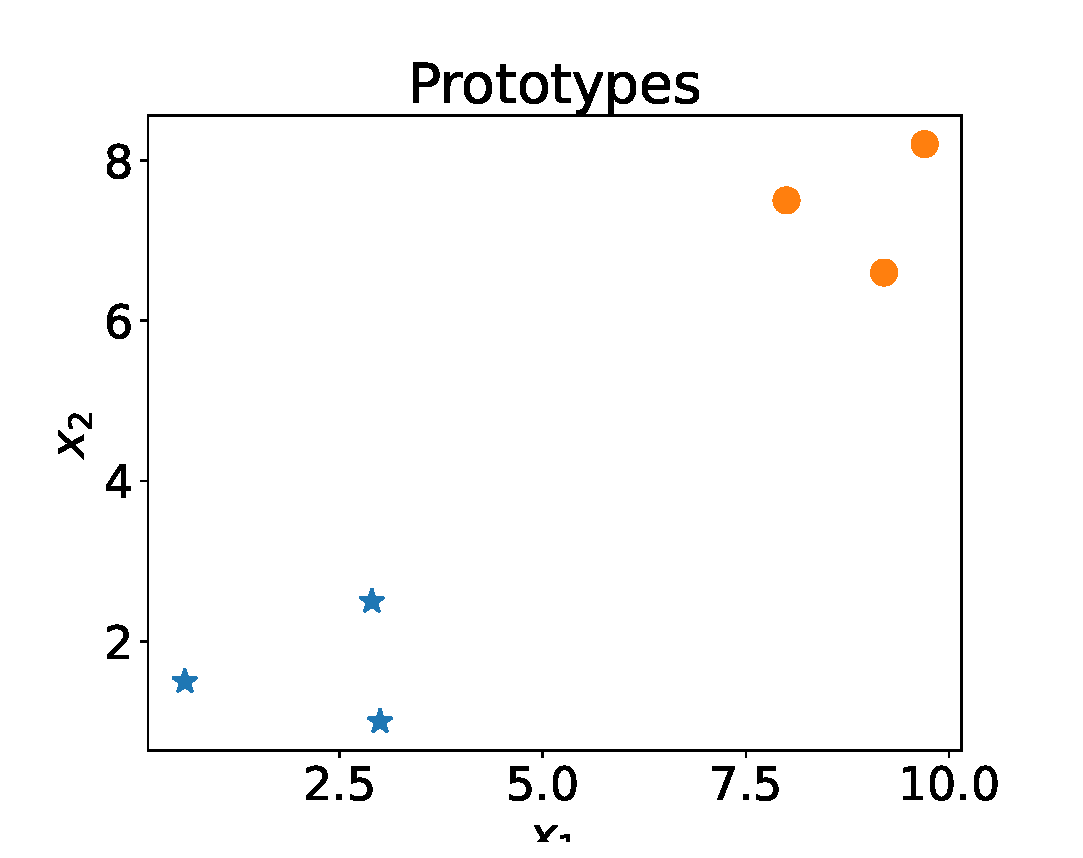
\includegraphics[width=.75\textwidth]{images/prototypes_0.eps}
  \caption{Prototypes of different categories}
  \label{fig:prototypes_0}
\end{figure}

We can also distinguish between two categories. For example, we could have a category of $\bigtriangleup$ and a category of $\bigcirc$.
Now, the question is: \textit{What do we do if we get a new data point?} For example $\vec{x}_{\times} = \begin{pmatrix}7.5\\4.0\end{pmatrix}$

\begin{figure}[h]
  \centering
  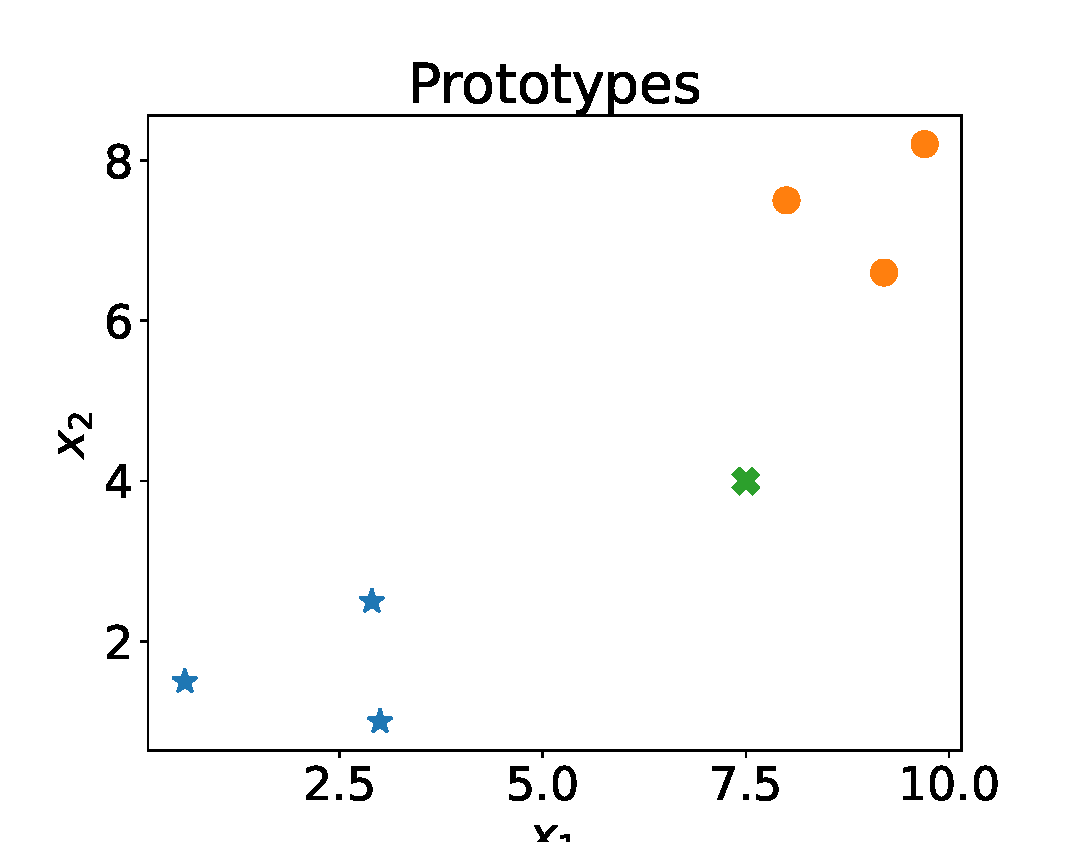
\includegraphics[width=.75\textwidth]{images/prototypes_1.eps}
  \caption{A new sample was added to the data set}
  \label{fig:prototypes_1}
\end{figure}

We need to find a mechanism of assigning a label to a new data point \textit{cross}.
For existing points we have this information already and we know which point belongs to which category. 
So how do we know which category the new point belongs to?

Psychiologists came up with the idea of designing so called \textit{prototypes} for each category.

This easiest solution for such prototype is calculating the \underline{mean} of all points in a category.
In this example we would compute the mean of all $\bigtriangleup$ $\vec{\mu}_\bigtriangleup$ and the mean of all $\bigcirc$ $\vec{\mu}_\bigcirc$.
\begin{figure}[h]
  \centering
  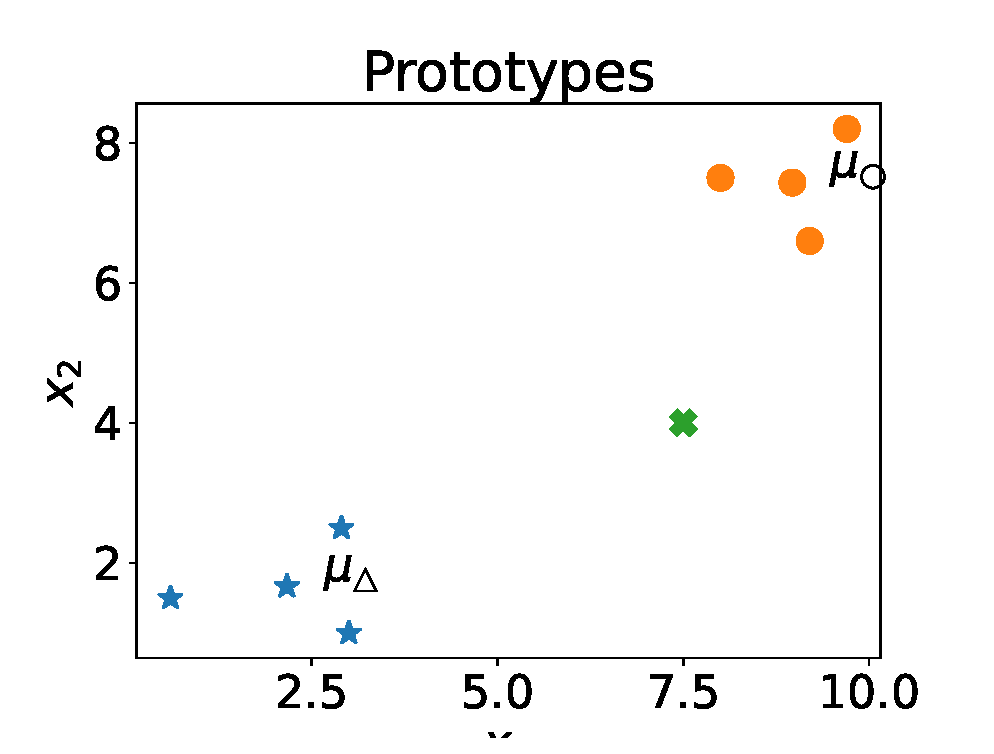
\includegraphics[width=.75\textwidth]{images/prototypes_2.eps}
  \caption{Mean values as prototypes for different categories are used to determine the label of a new data point}
  \label{fig:prototypes_2}
\end{figure}

The formula for the mean is:
\begin{equation}
  \vec{\mu} = \frac{1}{N} \sum_{i=1}^{N} x_i
  \label{eq:mean}
\end{equation}
where $N$ is the number of samples and $x_i$ is the $i$-th sample.
For each of the categories this translates to
\begin{align}
  \vec{\mu}_\bigtriangleup &= \frac{1}{N_\bigtriangleup} \sum_{i=1}^{N_\bigtriangleup} x_{\bigtriangleup, i} \\
  \vec{\mu}_\bigcirc &= \frac{1}{N_\bigcirc} \sum_{i=1}^{N_\bigcirc} x_{\bigcirc, i}
\end{align}
A label for a new data point $\vec{x}_{\times}$ can now be assigned by calculating the distance to each of the prototypes $\vec{\mu}_{\bigtriangleup}$ and $\vec{\mu}_{\bigcirc}$ and assigning the label of the prototype with the smallest distance.

One method to compute these distances is the \textbf{Euclidean Distance}, which is defined as
\begin{equation}
  d(\vec{x}, \vec{y}) = \sqrt{\sum_{i=1}^{N} (x_i - y_i)^2} = \sqrt{(\vec{x} - \vec{y})^T (\vec{x} - \vec{y})}
\end{equation}
where $n$ is the number of dimensions of the vectors $\vec{x}$ and $\vec{y}$.
There are many more distance metrics, and throughout this book we will encounter a few of them, but for now we will stick to the Euclidean Distance.
After computing all distances they can be compared and the label of the prototype with the smallest distance can be assigned to the new data point.
Mathematically this can be written as
\begin{equation}
  k^* = \argmin_{k\in\{1,\dots,K\}} d(\vec{x}, \vec{\mu}_k)
  \label{eq:nearest_centroid_inference}
\end{equation}
with $k^*$ being the label of the new data point $\vec{x}$ and $K$ being the number of categories.

\textbf{Congratulations!} You just implemented your first classification algorithm, the Nearest Centroid Classifier.
\section{Implementation}
In the following, we will look into different implementations of the NCC algorithm. And will look into two different approaches to compute the prototypes.
These two approaches can be used in most common Machine Learning algorithms.

\subsection{Inference}
The pseudo code to perform a classification (inference) using the NCC algorithm is very simple:
\begin{algorithm}
\LinesNumbered
\caption{\textbf{N}earest \textbf{C}entroid \textbf{C}lassifier Inference}\label{alg:ncc}
\KwData{$\vec{x}\in\mathbb{R}^D, \vec{\mu}_k, k\in\{1,\dots,K\}$}
\KwResult{$k^*$}
\Comment*[h]{Compute nearest class centroid}\\
$k^* \gets \argmin_{k\in\{1,\dots,K\}} d(\vec{x}, \vec{\mu}_k)$\;
\end{algorithm}

There are different ways to compute the centroids, here we used the means.
To compute the means we can use two different approaches, we call these approaches \textit{batch} and \textit{streaming}.
These terms might not 100\% match the common understanding of these terms, but we will use them to distinguish between the two approaches.

\textbf{Batched} refers to the fact that we compute the mean of all samples in a category at once. This approach requires
us to store all samples in memory and then compute the mean. This is the easier, but more expensive approach.

\textbf{Streaming} refers to the fact that we compute the mean of all samples in a category one by one. This approach does not require
us to store all samples in memory and is therefore more memory efficient. This approach is also called \textit{online} learning.

\subsection{Batched}
The batched approach is the easier one to implement. We simply store all samples in memory and then compute the mean.
\begin{algorithm}
\LinesNumbered
\caption{\textbf{NCC} Means (Batched)}\label{alg:ncc_batched}
\KwData{$\vec{x}\in\mathbb{R}^D, \vec{\mu}_k, k\in\{1,\dots,K\}$}
\KwResult{means $\vec{\mu}_k, k\in\{1\dots k\}$}
\Comment*[h]{Init means and counters for each class}\\
\Comment*[h]{Computation of class means}\\
\For{class $k$ in $K$}{
  $\vec{\mu}_k \gets \frac{1}{N_k}\sum^{N_k}_{i=1}\vec{x_i}$\;
}
\end{algorithm}

\subsection{Streaming}
To derive the streaming approach we need to look at the mathematical definition of the batched version
\begin{equation}
  \vec{\mu}_k = \frac{1}{N_k}\sum^{N_k}_{i=1}\vec{x_i}
\end{equation}
Imagine now, that we don't actually have the $N$-th data point yet.
We can rewrite the equation as
\begin{equation}
  \vec{\mu}_k = \frac{1}{N_k}\sum^{N_k-1}_{i=1}\vec{x_i} + \frac{1}{N_k}\vec{x_{N_k}}
\end{equation}
We can see the factor $\frac{1}{N_k}$ is the same for all terms. This factor can be rewritten a bit differently
\begin{equation}
  \frac{1}{N_k} = \frac{1}{N_k-1} \cdot \frac{N_k-1}{N_k}
\end{equation}
Now we can rewrite the equation as
\begin{equation}
  \vec{\mu}_k = \frac{1}{N_k}\sum^{N_k-1}_{i=1}\vec{x_i} + \frac{1}{N_k} \cdot \vec{x_{N_k}} = \frac{N_k - 1}{N_k}\frac{1}{N_k-1}\sum^{N_k-1}_{i=1}\vec{x_i} + \frac{1}{N_k} \cdot \vec{x_{N_k}}
\end{equation}
If we compare the middle term $\frac{1}{N_k}\sum^{N_k-1}_{i=1}\vec{x_i}$ with the original equation \eqref{eq:mean} we can see that it is just the mean of the previous iteration $\vec{\mu}_{k-1}$
\begin{equation}
  \Rightarrow \vec{\mu}_{k} = \frac{N_k - 1}{N_k}\vec{\mu}_{k-1} + \frac{1}{N_k} \cdot \vec{x_k}
  \label{eq:iterative-mean}
\end{equation}

This equation can be used to iteratively compute the mean of a category. We can start with $\vec{\mu}_0 = \vec{0}$ and then compute the mean of each sample by using the equation \eqref{eq:iterative-mean}.
An implementation of this approach is shown in Algorithm \ref{alg:ncc_streaming}.
\begin{algorithm}
\LinesNumbered
\caption{\textbf{NCC} Means (Streaming)}\label{alg:ncc_streaming}
\KwData{$\vec{x}\in\mathbb{R}^D$ labels $y_1, \dots, y_N\in\{1,\dots,K\}$}
\KwResult{means $\vec{\mu}_k, k\in\{1\dots k\}$}
\Comment*[h]{Init means and counters for each class}\\
$\forall k:$ $\vec{\mu}_k \gets \vec{0}, N_k = 0$\;
\For{Data point $i = 1,\dots,N$}{
  \Comment*[h]{Update means and counters}\\
  $k \gets y_i$\;
  $\vec{\mu}_k \gets \frac{N_k}{N_k + 1}\vec{\mu}_{k} + \frac{1}{N_k + 1} \cdot \vec{x_i}$\;
  $N_k \gets N_k + 1$\;
}
\end{algorithm}
As you can see for this iterative approach we only need to store all $\vec{\mu}_k$ and $N_k$ in memory. This is a huge advantage over the batched approach, especially if we have a lot of data.

You can see a visualization of the two approaches in Figure \ref{fig:ncc_batched_streaming}.

\section{Limitations}
Once we implemented one of the two approaches we can use it to classify new data points. For the example above this might result in \textit{Decision Boundaries} as shown in Figure \ref{fig:ncc_db_uncorrelated}.
This brings up a new group of questions, specifically about the limitations of the NCC or when 
should we use the NCC and when should we not use it.


The NCC is a very simple algorithm and therefore has some limitations.
\begin{enumerate}
  \item NCC should only be used for uncorrelated data, i.e. $x_1$ and $x_2$ are independent/without any correlation.
    The background here is the prediction by the model, the line between the two colors in Figure \ref{fig:ncc_db_uncorrelated} is called the \textit{Decision Boundary} (DB). We see that
    we have not a single miss-classification in this example. But this doesn't apply to all cases.
    Occasionally we will witness miss-classifications even in simple examples.
    This is due to the fact that the NCC is a linear classifier and therefore can only separate linearly separable data. Whenever we have \textit{outliers}, \textit{mislabeled data} or \textit{noise} in the input data, it is inevidable that the NCC will not be able to separate the data with full accuracy.
  \item The NCC does not consider correlation when classifying. It only computes and copares mean values of the data.\\
    Compare the decision boundaries in Figure \ref{fig:ncc_db_uncorrelated} and Figure \ref{fig:ncc_db_correlated}. In Figure \ref{fig:ncc_db_correlated} we see that the decision boundary is not optimal, several data points of the blue class would be classified as orange and vice versa.
    If we compute only the means, we can not successfully separate the correlated data with a single DB.
  \item This also applies to a problem with more than two classes. If we have more than two classes, we can not use a single DB to separate the data.
    We would need to compute multiple DBs to separate the data, as visualized in Figure \ref{fig:ncc_db_3_class}.
\end{enumerate}

\begin{figure}[h]
  \centering
  \begin{minipage}{.45\textwidth}
  \centering
    \includesvg[width=.95\textwidth]{images/NCC_uncorrelated.svg}
    \caption{Decision Boundaries for uncorrelated data}
    \label{fig:ncc_db_uncorrelated}
  \end{minipage}
  \hfill
  \begin{minipage}{.45\textwidth}
  \centering
    \includesvg[width=.95\textwidth]{images/NCC_correlated.svg}
    \caption{Decision Boundaries for correlated data}
    \label{fig:ncc_db_correlated}
  \end{minipage}\newline
  \hfill
  \begin{minipage}{.45\textwidth}
  \centering
    \includesvg[width=.95\textwidth]{images/NCC_3_class.svg}
    \caption{Decision Boundaries for 3 classes}
    \label{fig:ncc_db_3_class}
  \end{minipage}
  \hfill
\end{figure}

\section{Linear Classification}
\label{sec:linear_classification}
In the previous section we motivated the NCC by using a psychological model. We also saw that the NCC is good for uncorrelated data, data that is linear separable.\\
Under the hood the NCC is computing Decision Boundaries to separate the data, this DB is a line in the feature space.
This puts the NCC algorithm into the group of \textit{Linear Classifiers}. Linear Classifiers are a group of algorithms that perform well on linearly separable data, just like the NCC.
The NCC is a very simple linear classifier, but there are more complex ones. We will look into some of them in later chapters.
But what is this line that separates the data? How can we compute it?\\
We will look into this now in a more mathematical way.
\subsection{From Prototypes to Linear Classification}
Now we will use the definition of NCC \eqref{eq:nearest_centroid_inference} to derive general linear classification.
Let $\vec{x} \in \mathbb{R}^D$ be a data point and $\vec{\mu}_k \in \mathbb{R}^D$ be the prototype of class $k$. For two classes this would be $\vec{\mu}_0$ and $\vec{\mu}_1$.

Then we would find the class of $\vec{x}$ by computing the distance to each prototype and assigning the label of the prototype with the smallest distance.
\begin{equation}
  k^* = \argmin_{k\in\{1,\dots,K\}} d(\vec{x}, \vec{\mu}_k)
\end{equation}
or
\begin{align}
  k^* &= \argmin(d(\vec{x}, \vec{\mu}_0), d(\vec{x}, \vec{\mu}_1))\\
  \Leftrightarrow&\, d(\vec{x}, \vec{\mu}_0) > d(\vec{x}, \vec{\mu}_1)
\end{align}
This is the same as saying that $\vec{x}$ is closer to $\vec{\mu}_0$ than to $\vec{\mu}_1$. We can write this as
\begin{align}
  \Leftrightarrow& \norm{\vec{x} - \vec{\mu}_0}_2^2 > \norm{\vec{x} - \vec{\mu}_1}_2^2
\end{align}
where $\norm{\cdot}_2$ is the Euclidean norm. We can square both sides of the inequality and get
\begin{align}
  \Rightarrow& \norm{\vec{x} - \vec{\mu}_0}_2 > \norm{\vec{x} - \vec{\mu}_1}_2
\end{align}
We can now expand the Euclidean norm to get
\begin{align}
  \Rightarrow\, & \vec{x}^T\vec{x} - 2\vec{x}^T\vec{\mu}_0 + \vec{\mu}_0^T\vec{\mu}_0 > \vec{x}^T\vec{x} - 2\vec{x}^T\vec{\mu}_1 + \vec{\mu}_1^T\vec{\mu}_1 \\
  \Leftrightarrow\, & - 2\vec{x}^T\vec{\mu}_0 + \vec{\mu}_0^T\vec{\mu}_0 > - 2\vec{x}^T\vec{\mu}_1 + \vec{\mu}_1^T\vec{\mu}_1 \\
  \Leftrightarrow\, & \vec{\mu}_0^T\vec{x} - \frac{\vec{\mu}_0^T\vec{\mu}_0}{2} < \vec{\mu}_1^T\vec{x} - \frac{\vec{\mu}_1^T\vec{\mu}_1}{2} \\
  \Leftrightarrow\, & 0 < (\underbrace{\vec{\mu}_0-\vec{\mu}_1}_{\vec{\omega}})^T\vec{x} - \underbrace{\frac{1}{2}\left(\vec{\mu}_0^T\vec{\mu}_0-\vec{\mu}_1^T\vec{\mu}_1\right)}_{\beta}
\end{align}
$\vec{\omega}$ is called the \textit{weight vector}, for NCC this is the difference vector between both means.
$(\vec{\mu}_0-\vec{\mu}_1)^T\vec{x}$ is called the \textit{activation} of the input $\vec{x}$. From the previous chapter \ref{ch:math} we know that this is essentially just projecting $\vec{x}$ onto the difference vector, which will result in a constant value.
The constant value is then compared to the bias $\beta$ and if it is greater than $\beta$ the input is classified as class $0$, otherwise as class $1$.
In other words
\begin{equation}
  0 < \vec{\omega}^T\vec{x} + \beta
  \label{eq:linear_classifier}
\end{equation}
This is the general form of a linear classifier.
Using this general form we can now compute the DB for the NCC example

\begin{minipage}{.45\textwidth}
  {
  \centering
\begin{align}
  \vec{\tilde{x}} &= \left(\vec{{\omega}}^T\vec{x}\right) \\
  \vec{\tilde{x}} - \beta &= \left\{\begin{matrix}
    > 0 & \text{class } 0 \\
    < 0 & \text{class } 1
  \end{matrix}\right.
\end{align}
  }
with class $0$ the orange class and class $1$ the blue class.
\end{minipage}
\begin{minipage}{.45\textwidth}
  \centering
  \includesvg[width=.95\textwidth]{images/NCC_lin_classifier.svg}
  \caption{NCC as linear classifier, the blue line visualizes the decision boundary $\vec{\omega}$ and the green line is the decision threshold $\beta$}
  \label{fig:ncc_linear_classifier}
\end{minipage}
\vspace{1cm}

This is more or less all we need to know from linear classifiers and we can now derive it from the NCC algorithm.

\subsection{Linear Classification}
We will now look a bit deeper into linear classification.
Linear classification algorithms predict classes for given data points $\vec{x}$ by computing the activation of the input $\vec{x}$ and comparing it to a bias $\beta$
\begin{equation}
  f(\vec{x}) = \vec{\omega}^T\vec{x} + \beta
  \label{eq:linear_classification}
\end{equation}
where $\vec{\omega}$ is the decision boundary and $\beta$ is the decision threshold.
For two classes $\vec{\omega}$, the difference of the class means, is a vector and $\beta$ is a scalar
\begin{equation}
  \vec{\omega}_{\text{NCC}} = \vec{\mu}_0 - \vec{\mu}_1
\end{equation}
There are other ways to calculate $\vec{\omega}$ for other linear classifiers.
Using this definition we can build the NCC as a linear classification model
\begin{equation}
  f(\vec{x}) = \vec{\omega}_{\text{NCC}}^T\vec{x} + \beta_{\text{NCC}}
\end{equation}

What does this geometrically mean?\\
First, we assume our data is sepearable by the diagonal through the 2nd and 4th quadrant. This is the same as saying that the data is linearly separable and we won't need a threshold $\beta$ for now.
$\vec{\omega}$ is parallel to ${\vec{\mu}_0-\vec{\mu}_1}$ and therefore orthogonal to the DB.
Then any point above the DB, perpendicular to $\vec{\omega}$, will be classified as class $0$ and any point below the DB will be classified as class $1$. You can see a visualization of that in Figure \ref{fig:linear_classifier_origin}.

\begin{minipage}{.45\textwidth}
  \centering
  \includesvg[width=.95\textwidth]{images/linear_classifier_origin.svg}
  \caption{Linear Classifier without bias}
  \label{fig:linear_classifier_origin}
\end{minipage}
\hfill
\begin{minipage}{.45\textwidth}
  \centering
  \includesvg[width=.75\textwidth]{images/linear_classifier_origin_bias.svg}
  \caption{Linear Classifier with bias}
  \label{fig:linear_classifier_origin_bias}
\end{minipage}

Now, let's look at the bias value $\beta$. Figure \ref{fig:linear_classifier_origin_bias} demonstrates that the bias is the value that is added to the activation of the input $\vec{x}$.
You can literally say that we simply shift our DB up or down along the $x_2$-axis by $\beta$.


\framedtext{\color{red}{TODO:} Add more details about linear classification, add linear classifier plots}

\section{Implementation}
\framedtext{\color{red}{TODO:}}


\section{Example}
\framedtext{\color{red}{TODO:}}



\chapter{Nearest Neighbor Classifier}
\label{ch:knn}
\framedtext{\color{red}{TODO:}}



\chapter{Feature Extraction}
\label{ch:feature-extraction}
In this chapter we will talk about feature extraction, which is an essential part of any ML project/workflow.
We will introduce these by looking at a simple example and then look at some more advanced techniques.
After we covered most common approaches we will look into a very important concept, \underline{Machine Learning Pipelines}.

\section{Motivation}
Feature Extraction describes the transformations from any kind of data to vectors.
Until now, we always assumed to have a vector representation of our training data.
We used the notation of $\vec{x} \in \mathbb{R}^d$ to describe a $d$-dimensional data point.
To represent the full data set we used the convention $\vec{X} \in \mathbb{R}^{N \times d}$ 
a $N$-by-$d$ matrix, where each row represents a data point. This notation is commonly used among ML practitioners
and widely implemented in ML libraries. But it is not the only way to represent data. In fact, it is not even the most common way to represent data.
In this chapter we will look into different ways to represent data and how to transform data into a vector representation.

One of the most important things in solving a problem with an ML model is selecting correct features.
Most moder achievements in ML are not due to new algorithms, but due to better ways to extract features.
Thankfully, for most problems we do not need to use any fancy feature extraction techniques or bleeding edge research.
Classical, standard feature extraction techniques are sufficient to solve most problems in a satisfying manner.
In this chapter we will look into some of these techniques, but there are many more.
It is important to underline here, that often the best feature extractors are created by experts with domain knowledge.
Sometimes this expert can be you, but often it is not. In this case it is important to talk to the experts and understand the problem and challenges.
But for many problems and data types there are prebuild methods that we can apply without aquiring the domaing knowledge.
Imagine any work in the Natural Language Processing (NLP) field. It would be horribly bad if every ML practitioner would need to study linguistics prior
to working on an NLP problem.
Lastly, many of theses feature extraction techniques have to be optimized in order to achieve the best results possible. The easiest approach for this is trial and error.

In this chapter we look into four different types of data and different techniques how to extract features from them.

\section{Continuous Features}
Continuous features are the easiest to understand and to work with. They are also the most common type of data.
Continues data, is simply numerical data as real or integer values $x \in \mathbb{R}^d$. In many models continuous features are not required
to be transformed, because they can be used directly. But for some models it is benefitial to normalize continuous features.
For instance if we optimize our model with gradient descent (GD) or when we apply regularization to our model\footnote{Both of these ideas will be introduced in the future, but it is important to mention them here.}.

Given a feature $\vec{x} \in \mathbb{R}^d$ (analog for multivariant) there are several standard normalization options.
\subsection{Normalization: z-Score}
One of the normalization methods foro continuous features is the z-Score or standard scaling.
The z-Score is defined as
\begin{equation}
  z = \frac{x - \mu}{\sigma}
\end{equation}
where $\mu$ is the mean and $\sigma$ is the standard deviation of the feature.

In Python we can implement this as follows:
\begin{lstlisting}[language=Python, caption={z-Score in Python}, label={code:z-score}]
def z_score(X):
  return (X - X.mean(axis=0)) / X.std(axis=0)
\end{lstlisting}
Imagine the data set $\vec{X} \in \mathbb{R}^{N \times 1}$ ($N$ is the number of samples), then we can compute the mean of $\vec{X}$ through \lstinline{X.mean(axis=0)}.
Analogously this approach works for the multivariant case $\vec{X} \in \mathbb{R}^{N \times d}$.
The same applies for the standard deviation \lstinline{X.std(axis=0)}.
Putting everything together we get the z-Score for a data set $\vec{X}$ as implemented in \coderef{code:z-score}.
This method is also implemented in \lstinline{sklearn.preprocessing.StandardScaler}.
\subsection{Normalization: Min-Max-Scaling}
Another form of normalization is Min-Max-Scaling. 
The previous normalization method is great if your data is in the shape of a normal distribution.
If it isn't, you might as well chose Min-Max-Scaling, which ensures that the minimum values $\min(\vec{x})$ and maximum values $\max(\vec{x})$ of the scaled data are in a certain range, e.g. $[0, 1]$.
It does so by computing the min $\min(\vec{x})$ and max $\max(\vec{x})$ of the feature and then scaling the data as follows
\begin{equation}
  x_{scaled} = \frac{x - \min(\vec{x})}{\max(\vec{x}) - \min(\vec{x})}
\end{equation}
The resulting variable is in the range $[0, 1]$ or any other.
This method is also implemented in \lstinline{sklearn.preprocessing.MinMaxScaler}.
The implementation of the Min-Max-Scaling is very similar to the z-Score implementation in \coderef{code:z-score} and can be found in \coderef{code:min-max-scaling}.

\begin{lstlisting}[language=Python, caption={Min-Max-Scaling in Python}, label={code:min-max-scaling}]
def min_max_scaling(X):
  x_min = X.min(axis=0)
  return (
    (X - x_min)
    / (X.max(axis=0) - x_min)
  )
\end{lstlisting}

Similar to the unnormlized data, the normalized data can be used in any ML model.

\section{Categorical Features}
As mentioned earlier continues features often don't need to be trasnformed. But categorical features most certainly need to be transformed.
Categorical features are variables $x \in C$ where $C$ can be any finite set of $N$ values without implicit ordering, e.g.
\begin{itemize}
  \item $C = \{red, green, blue\}$
  \item $C = \{dog, cat, mouse, horse\}$
  \item $C = \{1, 2, 6, 4, 5, 3\}$
  \item $C \in \{\text{User.id}\}$
\end{itemize}
The last example is a bit special, because it is not a finite set. But it is still a categorical feature, because it is not a continues feature.
The first three examples are called \textit{nominal} categorical features, because there is no implicit ordering.
To use these features in a ML model we need to transform them into a vector representation.
Here we will introduce the technique of \textit{One-Hot-Encoding} (OHE) to transform categorical features into a vector representation, but there are also
other techniques like for neural networks so called \textit{Embeddings}.
\subsection{One-Hot-Encoding}
We assume we have a fixed set of categorical values, e.g. $C = \{red, green, blue\}$. Then to generate the one-hot-encoding we first need to compute the cardinality of $C$.
The cardinality of a set is the number of elements in the set. In our example the cardinality of $C$ is $|C| = 3$. This means we need to transform each categorical value into a row-vector of length $|C|$.
For each categorical value we create a vector of length $|C|$ and set the value of the corresponding index to $1$ and all other values to $0$, so that
\begin{itemize}
  \item $red \rightarrow \begin{pmatrix}1 & 0 & 0\end{pmatrix}$
  \item $green \rightarrow \begin{pmatrix}0 & 1 & 0\end{pmatrix}$
  \item $blue \rightarrow \begin{pmatrix}0 & 0 & 1\end{pmatrix}$
\end{itemize}
By doing that categories can be easily represented as vectors.
This is also implemented in \lstinline{sklearn.preprocessing.OneHotEncoder}.
An example for using this approach are bag-of-words vectors, which we will look into in a second.

\subsection{One-hot-Encoding: Problems}
One of the main problems of OHE is that the cardinality of the categorical feature needs to be estimated upfront, i.e. prior to creation of the OHE vectors.
Therefore new items/categories can not be represented. Moreover, we lose the information on similarity between the categories, e.g. "light-blue" is as different as "green" to "blue".

\textbf{Note} In many situations we will face mixtures of continuous and categorical features. Usually we need to apply different extraction methods
to single features to put together a general feature representation of a sample.
\section{Text Features}
The next data type we will look into is text data. Again, we have several options here and especially lately this data type enjoys great popularity and research.
We will look at one approach more closely and shortly touch a few others.
The approach we will focus on is Bag-of-Words (BoW), a simple yet still very powerful technique that is very similar to the one-hot-encoding.
\subsection{Bag-of-Words}
To create BoW-Features we count the word occurrences in the given text. They are basically histograms of word occurrences.

\textbf{Example} Imagine we have the following text
\begin{quote}
  "The tokenizer splits the text into tokens."
\end{quote}
Then we can create a BoW-Feature vector as follows

\begin{table}[h]
  \centering
  \begin{tabular}{|l|ccccccc|}
    \hline
    \textbf{Word} & the & tokenizer & splits & text & into & tokens & . \\
    \hline
    \textbf{Count} & 2 & 1 & 1 & 1 & 1 & 1 & 1 \\
    \hline
  \end{tabular}
  \caption{BoW-Feature vector}
  \label{tab:bow}
\end{table}

How does this work?
\begin{enumerate}
  \item split the text into "tokens", e.g. words
  \item build one-hot-like vector for all found words
  \item count the occurrences of each word inside the text
\end{enumerate}
In the BoW approach $x$ is the vector of word occurrences. The name of an dimension is the word assigned to it.
$\vec{x} \in \mathbb{N}^d$ where $d$ is the number of unique words, the \underline{word vocabulary}, in the text.
$d$ needs to be determined prior to starting and can become quite big, which we will discuss in the following.
\subsubsection{Problems}
BoW-Features only account for the word historgram and due to that most of the natural language structure is lost.
We lose for example the order of words, or context when processing multiple senteces at once.

Overall, BoW-Features are still very efficient and a reasonable approach.

\subsubsection{Model with N-Grams}
To overcome the issue of losing language structure we can apply a different way of tokenizing our text document.
Before we used word-tokens, with N-Grams we use sequences of words, specifically sequences of $N$ words.
E.g. Bi-Grams constst of two words
\begin{table}[h]
  \centering
  \begin{tabular}{|l|ccccc|}
    \hline
    \textbf{Word} & the tokenizer & tokenizer splits & splits the & the text & ...\\
    \hline
    \textbf{Count} & 1 & 1 & 1 & 1 & ... \\
    \hline
  \end{tabular}
  \caption{BoW-Feature Bi-Gram vector}
  \label{tab:bow-bi-gram}
\end{table}
If we would consider every combination of words the dimensionality of this new vector $\vec{x}$ will also significantly change, because we represent sequences of words instead of single words now.
For the Bi-Gram example we get $x \in \mathbb{N}^{d^2}$ where $d$ is the number of unique Bi-Grams in the text.
An implementation of BoW-Features is available in sklearn's \lstinline{sklearn.feature_extraction.text.CountVectorizer}.

\subsubsection{Character N-Grams}
We will briefly look into another approach to BoW-Features, which is using character N-Grams instead of word N-Grams.
This approach uses character sequences instead of word sequences. This approach is especially useful for languages with a rich morphology, e.g. German.
Another great application is for language independent models, e.g. for language detection.
Eseentially, we can select a tokenization method that fits our needs best, then transform these tokens into a BoW encoding.

\subsubsection{Term Frequency - Inverse Document Frequency (TF-IDF)}
One of the problems of using token occurrences is that natural language contains a lot of words that don't transfer information.
Frequently occurring words like "the" are often not meaningful and will be weighted down by the inverse document frequency.
Usually, we see a word-frequency distribution in the shape of the distribution shown in Figure \ref{fig:word-freq-dist}.

\begin{figure}[h]
  \centering
  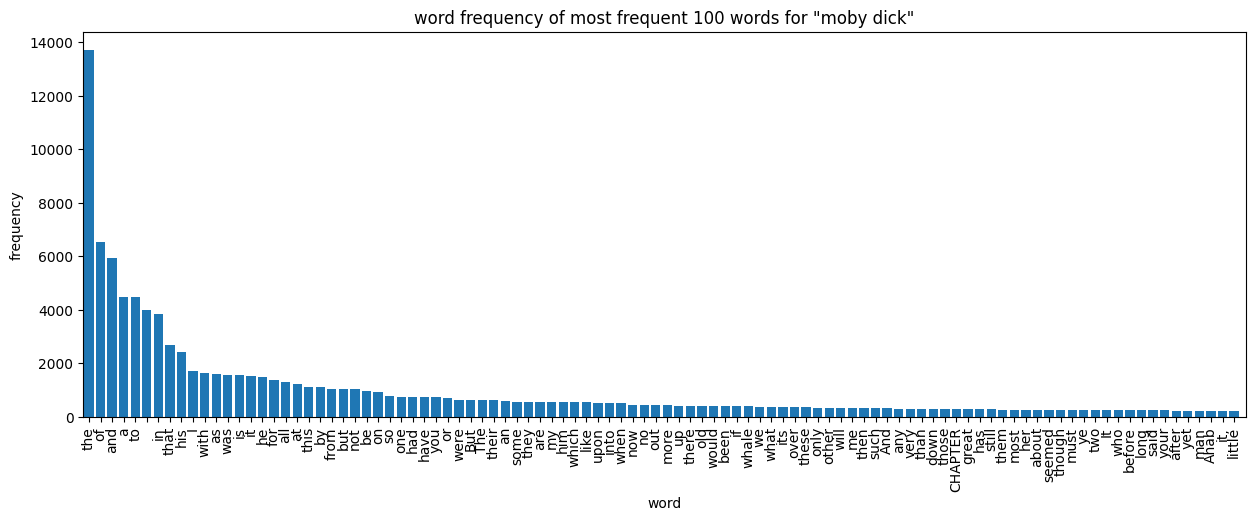
\includegraphics[width=.95\textwidth]{images/word-distribution.png}
  \caption{Word frequency distribution of 100 most frequent words in Moby Dick (https://www.gutenberg.org/ebooks/2701)}
  \label{fig:word-freq-dist}
\end{figure}
In order to downweight the frequently occurring words, to be able to only select relevant words, we apply the inverse
document frequency
\begin{equation}
  \text{idf}(t, d) = \log \frac{|d|}{|d \text{ containing } t|}
  \label{eq:IDF}
\end{equation}
This document frequency can be combined with the term frequency, the number of occurrences of a single word/token $|t|$ over the number of occurring words/tokens $|d|$
\begin{equation}
  \text{tf}(t, d) = \frac{|t|}{|d|}
  \label{eq:TF}
\end{equation}
tf \eqref{eq:TF} and idf \eqref{eq:IDF} can be combined by forming their product
\begin{equation}
  \text{tfidf}(t, d) = \text{tf}(t, d) \cdot \text{idf}(t, d)
  \label{eq:TF-IDF}
\end{equation}
A model incorporating this metric is TFIDF which is essentially a BoW model with applied term frequency and idf.

In sklearn you can find it under \lstinline{sklearn.feature_extraction.text.TfidfVectorizer}.

\subsubsection{Stop-Words}
Another alternative to remove noice from our data are Stop-Words.
Instead of computing tf and idf, we have a set of predefined words to exclude from the document.
For most languages we can do that and prepare a set of words that won't change frequently.
From my experience they seem to work great, and I use them more often than TF-IDF.

\subsubsection{Expensive N-Grams}
We quickly jump back to the N-Gram tokens and discuss the dimensionality of our BoW vectors.

If we use unigrams ($N = 1$) the size of our vectors $\vec{x} \in \mathbb{R}^d$ is $d$ the size of our vocabulary.
The size of this is $v$ in the worst case. Libraries use so called sparse vectors to represent these
high dimensional data points, dense representations require too much memory by storing $0$ values.
When we increase $N$ to $N=2$ (Bi-Grams) this memory requirement grows by a factor of $d$. So the worst case
scenario increases to $d^2 \Rightarrow \vec{x} \in \mathbb{R}^{d^2}$.
But mostly we do not gain much from this, in terms of increasing the context that is encoded.
This applies annalogously to higher orders of N-Grams, e.g. $N=3$ (Tri-Grams) require $V^3$ dimensions and so on.
If we consider e.g. German as a language, and we know that the vocabulary for this language is somewhere in the realm of $d \approx 10^{12}$.
This will cause big memory issues, especially when using anything else but Uni-Grams.

Before neural networks and deep learning google provided big sets of N-Gram data for many languages, so no one must create them
themself. You can find up to $N=5$-Grams here: \url{http://storage.googleapis.com/books/ngrams/books/datasetsv2.html}.

\subsubsection{Hashed N-Grams}
Another optimization trick to reduce memory of N-Grams is using hash-maps.

For those who know about hash-maps, instead of representing words/tokens as vectors, each dimension corresponds to a hash bucket
using a hash function.
This can cause hash-collision, a problem where two or more values are hashed to the same hash-value. It appears when the number of hash-buckets
is lower than the number of $N$-Grams we want to store.
But because of the structure of natural language we rarely have multiple senteces containing the same words in different orders, the collision rate is low to insignificant.
I highly encourage the reader to try it out, if you run out of memory with regular vectorizers.

For those of you who don't know about hash-maps, you can think of it as a dictionary, where each word is a key and the value is the number of occurrences, you can read more about
the inner workings of hash maps in the great 2020 blog post by Adam Gold \cite{adamgold:hash-maps}.

\subsubsection{Example \#1}
Let us look at an example of how to use these techniques in Python on a specific task.
We will use the 20 newsgroups data set, which is a collection of 20,000 newsgroup documents, partitioned (nearly) evenly across all newsgroups.
You can find more information about this data set here: \url{http://qwone.com/~jason/20Newsgroups/}.
Essentially, we will train a model to classify the newsgroup of a given document.
We will use the \lstinline{sklearn.datasets.fetch_20newsgroups} function to download the data set and then use the \lstinline{sklearn.feature_extraction.text.TfidfVectorizer}
to transform the text into a BoW representation.
After that we will train a NCC model and KNN model on the data set.
\begin{lstlisting}[language=Python, caption={20 newsgroups example}, label={code:20-newsgroups}]
from sklearn.datasets import fetch_20newsgroups
from sklearn.feature_extraction.text import TfidfVectorizer
from sklearn.neighbors import NearestCentroid, KNeighborsClassifier

# Download the data set
newsgroups_train = fetch_20newsgroups(subset='train')
newsgroups_test = fetch_20newsgroups(subset='test')

# Transform the text into a BoW representation
vectorizer = TfidfVectorizer()
X_train = vectorizer.fit_transform(newsgroups_train.data)
X_test = vectorizer.transform(newsgroups_test.data)

# Train a Nearest Centroid Classifier
clf = NearestCentroid()
clf.fit(X_train, newsgroups_train.target)
acc = (clf.predict(X_test) == imdb_test.target).mean()
print(f"Accuracy: {acc}")

# Train a KNN Classifier
clf = KNeighborsClassifier()
clf.fit(X_train, newsgroups_train.target)
acc = (clf.predict(X_test) == imdb_test.target).mean()
print(f"Accuracy: {acc}")
\end{lstlisting}

\begin{table}[h]
  \centering
  \begin{tabular}{|l|c|}
    \hline
    \textbf{Model} & \textbf{Accuracy} \\
    \hline
    \textbf{Nearest Centroid Classifier} & \textbf{0.692113648433351}\\
    K-Nearest Neighbors Classifier & 0.6591874668082847\\
    \hline
  \end{tabular}
  \caption{Accuracy of NCC and KNN on 20 newsgroups data set}
  \label{tab:20-newsgroups}
\end{table}

Running the code in \coderef{code:20-newsgroups} will result in the accuracy scores shown in Table \ref{tab:20-newsgroups}.
You will notice that albeit the simplicity of the NCC model it performs better than the KNN model. Furthermore, the NCC model is also substantially faster to train.

A better approach for this problem would be to use the Logistic Regression (LogReg) model. We will look into this model in the future (Chapter \ref{ch:regression}), for now we will consider it a black box and apply it to the news group data set to demonstrate its performance on this task.

\begin{lstlisting}[language=Python, caption={20 newsgroups example with Logistic Regression}, label={code:20-newsgroups-lr}]
from sklearn.datasets import fetch_20newsgroups
from sklearn.feature_extraction.text import TfidfVectorizer
from sklearn.linear_model import LogisticRegression

# Download the data set
newsgroups_train = fetch_20newsgroups(subset='train')
newsgroups_test = fetch_20newsgroups(subset='test')

# Transform the text into a BoW representation
vectorizer = TfidfVectorizer()
X_train = vectorizer.fit_transform(newsgroups_train.data)
X_test = vectorizer.transform(newsgroups_test.data)

# Train a Logistic Regression Classifier
clf = LogisticRegression(random_state=0)
clf.fit(X_train, newsgroups_train.target)
print(f"Accuracy: {clf.score(X_test, newsgroups_test.target)}")
\end{lstlisting}
\begin{table}[h]
  \centering
  \begin{tabular}{|l|c|}
    \hline
    \textbf{Model} & \textbf{Accuracy} \\
    \hline
    Nearest Centroid Classifier & 0.692113648433351\\
    K-Nearest Neighbors Classifier & 0.6591874668082847\\
    \textbf{LogisticRegression} & \textbf{0.8274030801911842}\\
    \hline
  \end{tabular}
  \caption{Accuracy of NCC, KNN and LogReg on 20 newsgroups data set}
  \label{tab:20-newsgroups-extended}
\end{table}
After running the code in \coderef{code:20-newsgroups-lr} we can see that the LogReg model performs significantly better than the NCC and KNN models (see Table \ref{tab:20-newsgroups-extended}).
This is due to the fact that the LogReg model is able to learn non-linear decision boundaries, which the NCC and KNN models are not able to do, because they are linear classifiers.
We will look into LogReg in the future, but for now it is important to understand that the NCC model is a linear classifier and therefore can only learn linear decision boundaries.
And apparently, the data set is not linearly separable, which is why the linear classification models perform so poorly.

\subsubsection{Example \#2}
In this example we will look into a different data set, the \textit{IMDB} data set~\cite{maas-EtAl:2011:ACL-HLT2011} (\url{http://ai.stanford.edu/~amaas/data/sentiment/}).
This data set contains 50,000 movie reviews from the Internet Movie Database, labeled by sentiment (positive/negative/unsupervised).
We will use the \lstinline{sklearn.datasets.load_files} function to download the data set and then use the \lstinline{sklearn.feature_extraction.text.TfidfVectorizer}
to transform the text into a BoW representation.
Similar to the previous example, we will classify the reviews using a NCC model and a LinReg model.

\begin{lstlisting}[language=Python, caption={IMDB example}, label={code:imdb}]
from sklearn.datasets import load_files
from sklearn.feature_extraction.text import TfidfVectorizer
from sklearn.neighbors import NearestCentroid
from sklearn.linear_model import LogisticRegression

# load the data set
imdb_train = load_files('aclImdb/train')
imdb_test = load_files('aclImdb/test')

# Transform the text into a BoW representation
vectorizer = TfidfVectorizer()
X_train = vectorizer.fit_transform(imdb_train.data)
X_test = vectorizer.transform(imdb_test.data)

# Train a Nearest Centroid Classifier
clf = NearestCentroid()
clf.fit(X_train, imdb_train.target)
print(f"Accuracy: {clf.score(X_test, imdb_test.target)}")

# Train a Logistic Regression Classifier
clf = LogisticRegression(random_state=42, solver='newton-cg', C=100.)
clf.fit(X_train, imdb_train.target)
acc = (clf.predict(X_test) == imdb_test.target).mean()
print(f"Accuracy: {acc}")
\end{lstlisting}
As the results in Table \ref{tab:imdb} show, the NCC model performs better on this task than the LogReg model.
\begin{table}[h]
  \centering
  \begin{tabular}{|l|c|}
    \hline
    \textbf{Model} & \textbf{Accuracy} \\
    \hline
    \textbf{Nearest Centroid Classifier} & \textbf{0.62312}\\
    Logistic Regression & 0.19984\\
    \hline
  \end{tabular}
  \caption{Accuracy of NCC and LogReg on IMDB data set}
  \label{tab:imdb}
\end{table}
But an accuracy of 62.31\% is not very good, especially considering that a random guess would result in an accuracy of 33.3\%.
One option would be to reduce the problem to a binary classification problem, i.e. positive or negative sentiment.
Doing so would result in an accuracy of 62.89\% for the NCC model and 17.56\% for the LogReg model.
As you can see, the NCC model still performs better than the LogReg model, but still not very good, frankly the improvement was rather sobering.

To improve on the $\approx 60\%$ accuracy we could use a different model architecture, e.g. a neural network.
In future chapters we will look closer into the architecture powering so called Multi-Layer Perceptrons (MLPs).
But for now it is important to understand that MLPs are able to learn non-linear decision boundaries, which is why they are able to perform better on this task.

Implementing an MLP is as easy as replacing the NCC model with a MLP model from the \lstinline{sklearn.neural_network.MLPClassifier} class.
\begin{lstlisting}[language=Python, caption={IMDB example with MLP}, label={code:imdb-mlp}]
from sklearn.datasets import load_files
from sklearn.feature_extraction.text import TfidfVectorizer
from sklearn.neural_network import MLPClassifier

# load the data set
imdb_train = load_files('aclImdb/train')
imdb_test = load_files('aclImdb/test')

# Transform the text into a BoW representation
vectorizer = TfidfVectorizer()
X_train = vectorizer.fit_transform(imdb_train.data)
X_test = vectorizer.transform(imdb_test.data)

# Train a MLP Classifier
clf = MLPClassifier(
  hidden_layer_sizes=(100, 100),
  max_iter=10,
  alpha=1e-4,
  solver='sgd',
  verbose=10,
  random_state=42,
  learning_rate_init=.1
)
clf.fit(X_train, imdb_train.target)
acc = (clf.predict(X_test) == imdb_test.target).mean()
print(f"Accuracy: {acc}")
\end{lstlisting}
The results in Table \ref{tab:imdb-mlp} show that the MLP model performs significantly better than the NCC and LogReg models.

\begin{table}[h]
  \centering
  \begin{tabular}{|l|c|}
    \hline
    \textbf{Model} & \textbf{Accuracy} \\
    \hline
    Nearest Centroid Classifier & 0.62312\\
    Logistic Regression & 0.19984\\
    \textbf{MLP Classifier} & \textbf{0.849}\\
    \hline
  \end{tabular}
  \caption{Accuracy of NCC, LogReg and MLP on IMDB data set}
  \label{tab:imdb-mlp}
\end{table}
Great, we were able to improve the accuracy from $\approx 60\%$ to $\approx 85\%$.

But this can't be it. We can do better than that. And we will.

A more advanced technique is to use word embeddings, which we will look into now.
\subsection{Word Embeddings}
The following section describes techniques which apply neural networks to generate word embeddings.
For now, we will look into how to use these embeddings as feature extractors.
Later, in Chapters \ref{ch:neural-networks} and \ref{ch:deep-learning}, we will look into how to train these embeddings models and how to use them for other tasks.
Word embeddings are a more advanced technique to represent words as vectors as the previosuly introduced OHE approach of BoW.\\
Over the past two years word embeddings have enjoyed great popularity and research among the ML community.
Especially with the rise of Large Language Models (LLMs) like BERT\cite{devlin2019bert} and GPT-3\cite{brown2020language}, the introduction of ChatGPT\cite{ChatGPT:2022} in late 2022 and the groundbreaking Open Source community around architectures of 2023 like LLaMa\cite{touvron2023llama}, LLaMa2\cite{touvron2023llama2} and Mixtral\cite{mixtral:2023}, these vectors became more and more relevant.

They are a dense representation of words, which means that they do not contain many $0$ values.
This is in contrast to the sparse representation of BoW-Features, which contain many $0$ values.
Word embeddings are usually trained on a large corpus of text, e.g. Wikipedia, and then used as a feature extractor for other tasks.
The most popular word embedding is the \textit{Word2Vec} embedding, which is trained on a large corpus of text coming from Wikipedia.
Word Embeddings are quite versatile, they can be used for many different tasks, e.g. word similarity, word analogies, text classification, etc.
We will look into the word similarity and word analogy tasks in a future chapter.
The quintessence of Word Embeddings is that they are able to encode semantic and syntactic information of words.
The most prominent example to demonstrate this encoded information is the following.

Let the embedding vector for the word "King" be $\vec{a} = \begin{pmatrix}1 & 1 & 0\end{pmatrix}$, the embedding vector of the word "Man" $\vec{b} = \begin{pmatrix}1 & 0 & 0\end{pmatrix}$ and the embedding vector for the word "Woman" be $\vec{c} = \begin{pmatrix}0 & 0 & 1\end{pmatrix}$.
  Then we can compute the embedding vector for the word "Queen" $\vec{d}$ by subtracting "Man" from "King" and adding "Woman" to create $\vec{d} = a - b + c = \begin{pmatrix}0 & 1 & 1\end{pmatrix}$.

This is of course a great simplification of the actual process. Embedding vectors have way more than just 3 dimensions and will most likely not contain beautiful integers as in this example.

We will look in Chapter \ref{ch:pca} into a technique called Principal Component Analysis (PCA), which can be used to reduce the dimensionality of embedding vectors to 2 or 3 dimensions. 
This allows us to visualize these high dimensional vectors.

You can check out \url{https://projector.tensorflow.org/} for a great visualization of word embeddings.

\subsubsection{Word2Vec}
Word2Vec is a word embedding technique that was introduced in 2013 by Mikolov et al. \cite{mikolov2013efficient}.
The idea behind Word2Vec is to train a neural network to predict the context of a word.
The context of a word is defined as the words surrounding the word in a given text.
The neural network is trained on a large corpus of text, e.g. Wikipedia, and then used as a feature extractor for other tasks.
A library that implements Word2Vec is \lstinline{gensim} \\(\url{https://radimrehurek.com/gensim/}).
Using Word2Vec is as easy as downloading a pre-trained model and then using it as a feature extractor.
\begin{lstlisting}[language=Python, caption={Word2Vec example}, label={code:word2vec}]
import gensim.downloader as api

# Download the pre-trained model
model = api.load("word2vec-google-news-300")

# Get the embedding vector for the word "King"
print(model["king"])
\end{lstlisting}
The code in \coderef{code:word2vec} will download the pre-trained Word2Vec model ($\approx$1.7 GB) from Google and then print the embedding vector for the word "King".

As you can see, we can generate embeddings for single words, but also for sentences and even paragraphs.Albeit the flexibility of the Word2Vec model, the model is not capable of generating embeddings for unknown words, i.e. words that are not in the original training vocabulary, e.g. "Kinging" and "Queening". 
This is a problem that is solved by the FastText model, which we will look into in the next section.

\subsubsection{FastText}
FastText is a word embedding technique that was introduced in 2016 by Bojanowski et al. \cite{bojanowski2016enriching}.
The idea behind FastText is to train a neural network to predict the context of a word, similar to Word2Vec.
But instead of using words as the smallest unit, FastText uses character N-Grams.
This allows FastText to generate embeddings for unknown words, i.e. words that are not in the original training vocabulary, e.g. "Kinging" and "Queening".
Gensim also provides a FastText model, which can be used in the same way as the Word2Vec model.
\begin{lstlisting}[language=Python, caption={FastText example}, label={code:fasttext}]
import gensim.downloader as api

# Download the pre-trained model
model = api.load("fasttext-wiki-news-subwords-300")

# Get the embedding vector for the word "King"
print(model["king"])
\end{lstlisting}
The code in \coderef{code:fasttext} will download the pre-trained FastText model ($\approx$1 GB) from Wikipedia and then print the embedding vector for the word "King".

\subsubsection{GloVe}
Another word embedding technique is GloVe, which was introduced in 2014 by Pennington et al. \cite{pennington2014glove}.
Other than FastText and Word2Vec, GloVe is not a neural network based model, but a matrix factorization technique.
The idea behind GloVe is to factorize the word-word co-occurrence matrix.
The word-word co-occurrence matrix is a matrix that contains the number of times a word $i$ appears in the context of word $j$.
The GloVe model is also available in Gensim.
\begin{lstlisting}[language=Python, caption={GloVe example}, label={code:glove}]
import gensim.downloader as api

# Download the pre-trained model
model = api.load("glove-wiki-gigaword-300")

# Get the embedding vector for the word "King"
print(model["king"])
\end{lstlisting}
The code in \coderef{code:glove} will download the pre-trained GloVe model ($\approx$1.4 GB) from Wikipedia and then print the embedding vector for the word "King".

\subsubsection{Comparison}
Now that we have looked into three different word embedding techniques, let us compare them.
We will use the same example as in the previous section, the 20 newsgroups data set.
We will use the \lstinline{sklearn.datasets.fetch_20newsgroups} function to download the data set and then use the embedding models to transform the text into a vector representation.
After that we will train a NCC model and MLP model on the data set.

\framedtext{\color{red}{TODO:} Code sample not working, fix it}

\begin{lstlisting}[language=Python, caption={20 newsgroups example with embeddings}, label={code:20-newsgroups-embeddings}]
from sklearn.datasets import fetch_20newsgroups
from sklearn.neighbors import NearestCentroid
from sklearn.neural_network import MLPClassifier
import gensim.downloader as api

# Download the data set
newsgroups_train = fetch_20newsgroups(subset='train')
newsgroups_test = fetch_20newsgroups(subset='test')

# Download the pre-trained models
word2vec_model = api.load("word2vec-google-news-300")
fasttext_model = api.load("fasttext-wiki-news-subwords-300")
glove_model = api.load("glove-wiki-gigaword-300")

# Transform the text into a vector representation
X_train_word2vec = [word2vec_model[x] for x in newsgroups_train.data]
X_test_word2vec = [word2vec_model[x] for x in newsgroups_test.data]
# Train a Nearest Centroid Classifier
clf = NearestCentroid()
clf.fit(X_train_word2vec, newsgroups_train.target)

# Train a MLP classifier
clf = MLPClassifier(
  max_iter=10,
  verbose=10,
  random_state=42,
)
clf.fit(X_train_word2vec, newsgroups_train.target)

print("Word2Vec")
print(f"NCC Accuracy: {clf.score(X_test_word2vec, newsgroups_test.target)}")
print(f"MLP Accuracy: {(clf.predict(X_test_word2vec) == newsgroups_test.target).mean()}")

del X_train_word2vec, X_test_word2vec

X_train_fasttext = [fasttext_model[x] for x in newsgroups_train.data]
X_test_fasttext = [fasttext_model[x] for x in newsgroups_test.data]

# Train a Nearest Centroid Classifier
clf = NearestCentroid()
clf.fit(X_train_fasttext, newsgroups_train.target)

# Train a MLP classifier
clf = MLPClassifier(
  max_iter=10,
  verbose=10,
  random_state=42,
)
clf.fit(X_train_fasttext, newsgroups_train.target)

print("FastText")
print(f"NCC Accuracy: {clf.score(X_test_fasttext, newsgroups_test.target)}")
print(f"MLP Accuracy: {(clf.predict(X_test_fasttext) == newsgroups_test.target).mean()}")
del X_train_fasttext, X_test_fasttext

X_train_glove = [glove_model[x] for x in newsgroups_train.data]
X_test_glove = [glove_model[x] for x in newsgroups_test.data]

# Train a Nearest Centroid Classifier
clf = NearestCentroid()
clf.fit(X_train_glove, newsgroups_train.target)

# Train a MLP Classifier
clf = MLPClassifier(
  max_iter=10,
  verbose=10,
  random_state=42,
)
clf.fit(X_train_glove, newsgroups_train.target)

print("GloVe")
print(f"NCC Accuracy: {clf.score(X_test_glove, newsgroups_test.target)}")
print(f"MLP Accuracy: {(clf.predict(X_test_glove) == newsgroups_test.target).mean()}")
\end{lstlisting}
The code in \coderef{code:20-newsgroups-embeddings} will download the pre-trained embedding models and then transform the text into a vector representation.
After that we train a NCC model and MLP model on the data set.

\section{Image Features}
We discussed until now continuous and categorical features, as well as text features.
To complete this we will briefly look at methods to extract features from images.
Due to the complexity of these methods we will only motivate them, because thoroughly understanding them would go beyond the scope of this book.
Most of them are very easy to use, but hard to understand.

\subsection{Classic Computer Vision}
Before 2012 (ImageNet Moment) researches used classic CV methods to extract features from images.
Mostly Furrier Decomposition was applied, this measures spacial frequencies of patches of the image.
The resulting frequency strength of each patch is then used as a feature.
These spacial frequencies are gradients in the image. High spacial frequencies are edges,
and the phase of the frequency is its orientation.
These kind of features are computed in the \underline{Histogram of Oriented Gradients/Edges} (HOG) feature extractor, as showcased in 
Figure \ref{fig:hog}.

\begin{figure}[h]
  \centering
  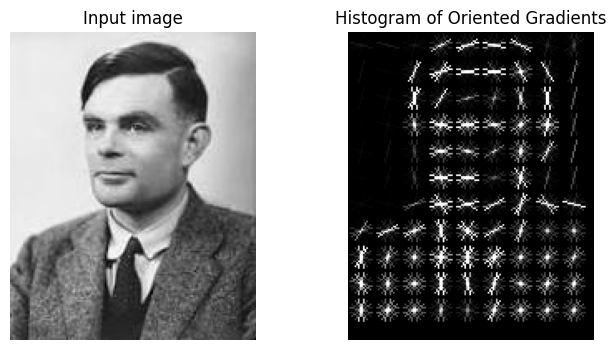
\includegraphics[width=.95\textwidth]{images/hog.png}
  \caption{HOG feature extraction}
  \label{fig:hog}
\end{figure}

HOG suits very well for object detection, because it is very robust to changes in illumination and other factors.
For this reason it is widely used in e.g. self-driving cars for pedestrian recognition.
They work good if we only want to encode a shape, e.g. a pedestrian, but not for more complex tasks like face recognition.
In skimage you can find the HOG extractor in \lstinline{skimage.feature.hog}.

\subsection{Convolutional Neural Networks}
Another more modern way of dealing with images is using Convolutional Neural Networks (CNNs).
They are state-of-the-art (SOTA) for image classification and object detection.
We don't have much time to look detaied into them, but the key takeaway here is:

We won't train these models from scratch. We will apply pretrained models, because we won't
be able to achieve same performance with models we would train ourselves.
And we don't want to spend so much time and money on training these models.
Thankfully, we don't need to because there are many pretrained models publicly available.
These models are trained foro a long time on very large datasets, e.g. ImageNet\cite{deng2009imagenet}, for us!
All we have to do is to download these models and run them as feature extractors.
You can read more about CNNs in \cite{PhilippZettl:2022} or Chapter \ref{ch:neural-networks}.


Essentially, CNNs are combinations of convolutional filter masks that are stacked on top of each other adding more and more complexity to the model.
The first layers learn simple features like edges and the last layers learn more complex features like shapes and objects.
The last layers are then used as features for our ML model.
Originally, when using the ImageNet data set, the models are trained on the image classification task.
But we can use the features of the last layers for any other task, e.g. object detection, because the features are still very meaningful and valid.
Instead of using the full pretrained model, we can also use only the first layers of the model and train the last layers on our own data set, or we simply
only use the first few pretrained layers as feature extractors.

You can see the representation of different channels from a specific layer in Figure \ref{fig:cnn-features} as well as the combination of all channels in Figure \ref{fig:cnn-features-1}.

\begin{figure}[h]
  \centering
  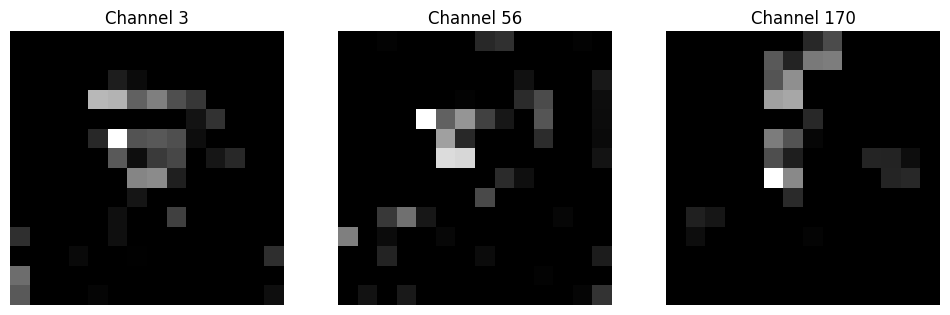
\includegraphics[width=.95\textwidth]{images/cnn-0.png}
  \caption{CNN feature extraction of different channels}
  \label{fig:cnn-features}
\end{figure}

\begin{figure}[h]
  \centering
  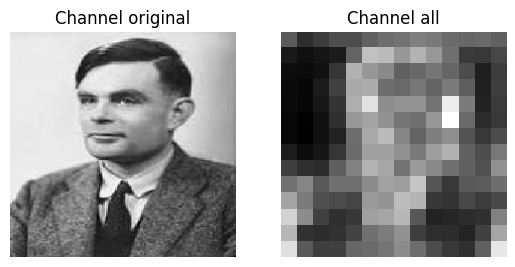
\includegraphics[width=.95\textwidth]{images/cnn-1.png}
  \caption{CNN feature channels combined}
  \label{fig:cnn-features-1}
\end{figure}

You can imagine image channels as a encoding of spacial frequencies, similar to the HOG features.
But other than HOG features, CNNs are able to learn these features in a general way by themselves, which is why they are so powerful.

Consider this, color images have three channels, red, green and blue. Each of these channels encodes a different spacial frequency.
Let $X \in \mathbb{R}^{H \times W \times 3}$ be an image with height $H$, width $W$ and three channels and random content (see Figure \ref{fig:channels}).
Then we can define three matrices $T_{red}, T_{green}, T_{blue} \in \mathbb{R}^{H \times W \times 3}$ that select the corresponding channel of each pixel.
\begin{align}
  \begin{pmatrix}
    \{\vec{x}_{1,1,1},\vec{x}_{1,1,2},\vec{x}_{1,1,3}\}
    & \{\vec{x}_{1,2,1},\vec{x}_{1,2,2},\vec{x}_{1,2,3}\}
    & \dots
    & \{\vec{x}_{1,W,1},\vec{x}_{1,W,2},\vec{x}_{1,W,3}\} \\
    \{\vec{x}_{2,1,1},\vec{x}_{2,1,2},\vec{x}_{2,1,3}\}
    & \{\vec{x}_{2,2,1},\vec{x}_{2,2,2},\vec{x}_{2,2,3}\}
    & \dots
    & \{\vec{x}_{2,W,1},\vec{x}_{2,W,2},\vec{x}_{2,W,3}\} \\
    \vdots & \vdots & \ddots & \vdots \\
    \{\vec{x}_{H,1,1},\vec{x}_{H,1,2},\vec{x}_{H,1,3}\}
    & \{\vec{x}_{H,2,1},\vec{x}_{H,2,2},\vec{x}_{H,2,3}\}
    & \dots
    & \{\vec{x}_{H,W,1},\vec{x}_{H,W,2},\vec{x}_{H,W,3}\}
  \end{pmatrix}
\end{align}
Then we can extract the three channels as follows.
For the red channel we select the first channel of each pixel
\begin{align}
  T_{red} = \begin{pmatrix}
    \{1, 0, 0\}
    & \{1, 0, 0\}
    & \dots
    & \{1, 0, 0\}\\
    \{1, 0, 0\}
    & \{1, 0, 0\}
    & \dots
    & \{1, 0, 0\}\\
    \vdots & \vdots & \ddots & \vdots \\
    \{1, 0, 0\}
    & \{1, 0, 0\}
    & \dots
    & \{1, 0, 0\}
  \end{pmatrix}
\end{align}
For the green channel we select the second channel of each pixel
\begin{align}
  T_{green} = \begin{pmatrix}
    \{0, 1, 0\}
    & \{0, 1, 0\}
    & \dots
    & \{0, 1, 0\}\\
    \{0, 1, 0\}
    & \{0, 1, 0\}
    & \dots
    & \{0, 1, 0\}\\
    \vdots & \vdots & \ddots & \vdots \\
    \{0, 1, 0\}
    & \{0, 1, 0\}
    & \dots
    & \{0, 1, 0\}
  \end{pmatrix}
\end{align}
And for the blue channel we select the third channel of each pixel
\begin{align}
  T_{blue} = \begin{pmatrix}
    \{0, 0, 1\}
    & \{0, 0, 1\}
    & \dots
    & \{0, 0, 1\}\\
    \{0, 0, 1\}
    & \{0, 0, 1\}
    & \dots
    & \{0, 0, 1\}\\
    \vdots & \vdots & \ddots & \vdots \\
    \{0, 0, 1\}
    & \{0, 0, 1\}
    & \dots
    & \{0, 0, 1\}
  \end{pmatrix}
\end{align}

Applying those three matrices to our image $X$ we get three images $X_{red}, X_{green}, X_{blue} \in \mathbb{R}^{H \times W \times 3}$ as individually shown in Figure \ref{fig:channels-individual}.
\begin{figure}
  \centering
\begin{minipage}[t]{.3\textwidth}
  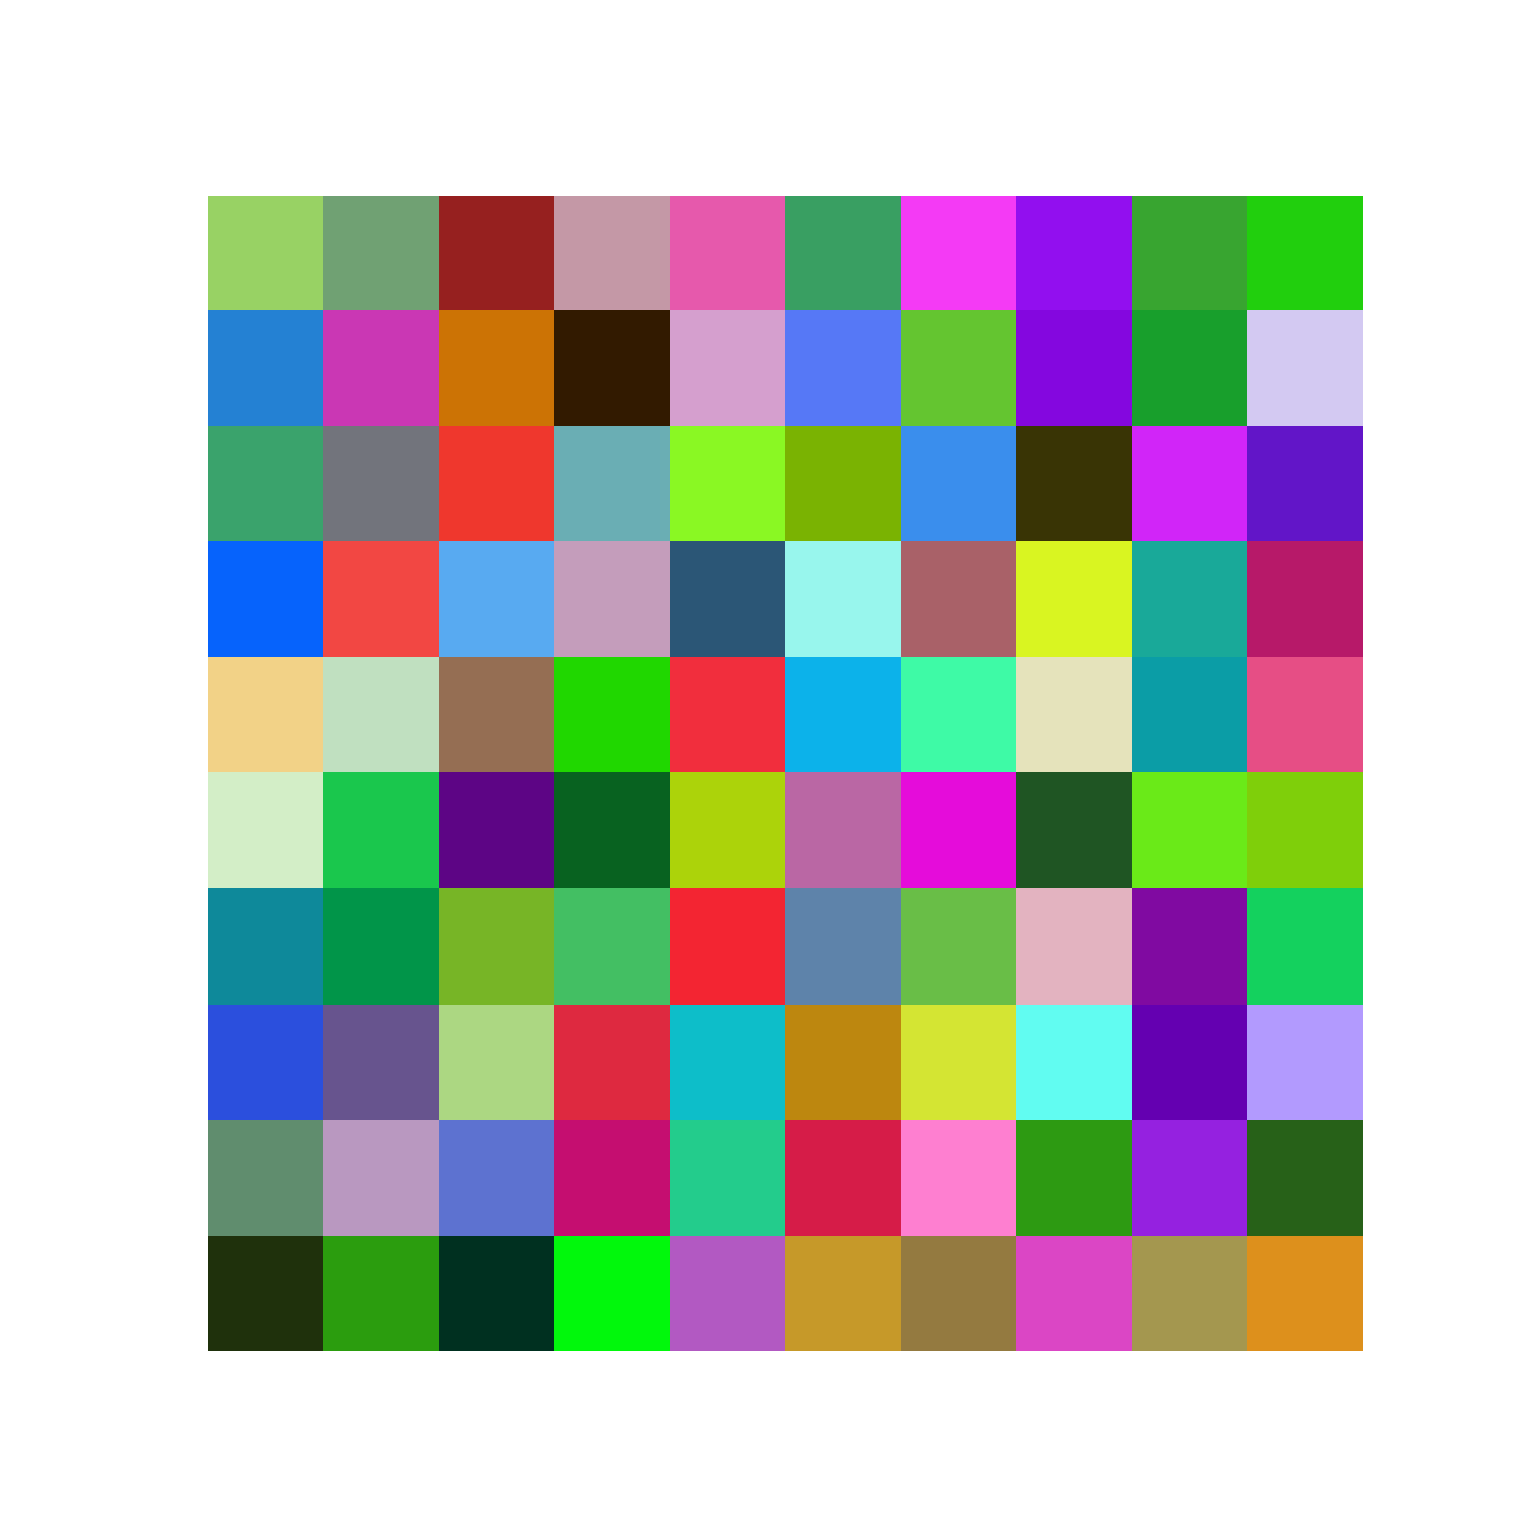
\includegraphics[width=.95\textwidth]{images/FE_img_rng_image.eps}
  \caption{Random image}
  \label{fig:channels}
\end{minipage}
\begin{minipage}[t]{.6\textwidth}
  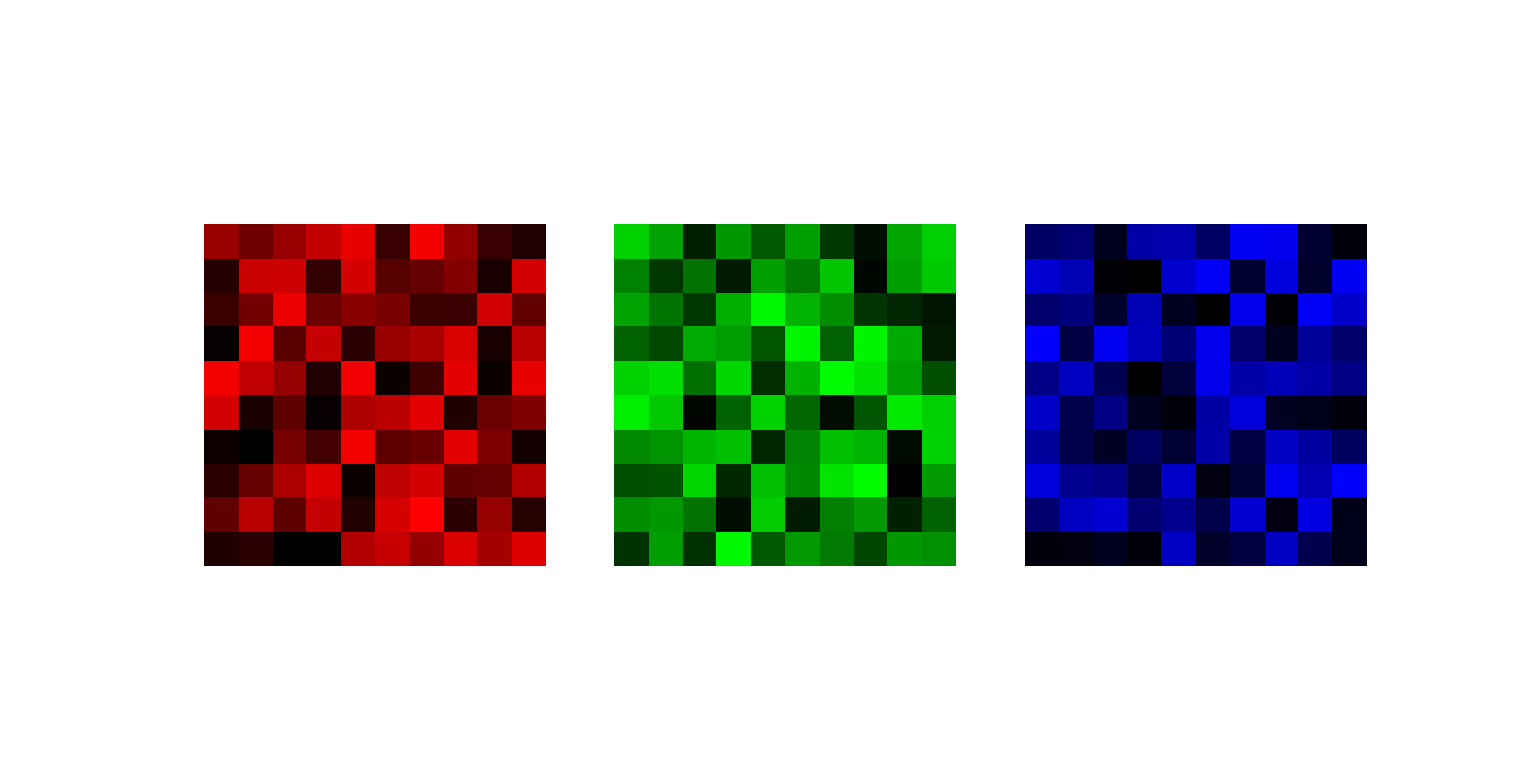
\includegraphics[width=.95\textwidth]{images/FE_img_channels.eps}
  \caption{Image channels individually}
  \label{fig:channels-individual}
\end{minipage}
\end{figure}

\framedtext{\color{red}{TODO:}} Implement example for CNN feature extraction



\chapter{Machine Learning Pipelines}
Recall the pipeline diagram from the first chapter.

\begin{figure}[h]
  \centering
  \begin{tikzpicture}
    \node[draw, rectangle] (data) at (0, 0) {Data};
    \node[draw, rectangle] (features) at (2.5, 0) {\begin{tabular}{c}Feature\\Extraction\end{tabular}};
    \node[draw, rectangle, minimum height=2cm, minimum width=6.25cm] () at (4.25, 0) {};
    \node[draw, rectangle] (model) at (6, 0) {\begin{tabular}{c}ML Model\\$f(x)$\end{tabular}};
    \node[draw, rectangle] (prediction) at (9, 0) {Prediction};
    \draw[->] (data) -- (features);
    \draw[->] (features) -- (model);
    \draw[->] (model) -- (prediction);
  \end{tikzpicture}
  \caption{Machine Learning Pipeline}
  \label{fig:ml-pipeline}
\end{figure}
Up until now we always assumed to have a vector representation $\vec{x}\in\mathbb{R}^d$ of our data.
Starting from now, our data might be in any other format, like text or images.

To build a system that gets a certain format of input, transform this input into $d$ dimensional vectors and feeds them into our model.
We will now look at how to program such an ML-Pipeline
\section{Motivation}
In the previous chapters we looked into different feature extraction techniques.
We also looked in previous chapters into different ML models and how to train them.
Now, we will look into how to combine these two concepts into a single pipeline.

One way how to implement this is to manually write code that executes all steps of the pipeline sequentially.
But this would be quite static and not very flexible. We would need to rewrite the code for every new data set or whenever
we want to change a part of the pipeline.

A better way to implement this is to use a so called \textit{Pipeline} object. This object is a wrapper around all steps of the pipeline.
The most popular API-Interface~\cite{sklearn_api} for this is implemented by the guys from scikit-learn~\cite{scikit-learn}.

We will look into the implementation of such a pipeline in the following because it will allow to combine
own implementations with implementations inside scikit-learn. This is especially useful because scikit-learn
delivers plenty of tools, feature extraction algorithms and model architectures.

I personally work a lot with scikit-learn and I highly recommend it to anyone who wants to get started with ML as well assigned
encourage everyone to contribute to the project.

\section{Estimators}
\framedtext{\color{red}{TODO:}}




\chapter{Metrics}
\framedtext{\color{red}{TODO:}}
\chapter{Model Evaluation}
\label{ch:model-evaluation}
\framedtext{\color{red}{TODO:}}

\chapter{Perceptron}
\label{ch:perceptron}
Perceptrons are among KNN and NCC one of the simplest, yet powerful and popular algorithms. They are the easiest form of Neural Networks
that we know of and are a great introduction into the field of Artificial Neural Networks.

But first we make a small recap of the NCC algorithm. Remember, we defined the prototypes corresponding to each class as the means
\begin{align}
  \vec{\mu}_{\triangle} = \frac{1}{N_{\triangle}} \sum_{\vec{x} \in \mathcal{X}_{\triangle}} \vec{x}\\
  \vec{\mu}_{\circ} = \frac{1}{N_{\circ}} \sum_{\vec{x} \in \mathcal{X}_{\circ}} \vec{x}
\end{align}
to classify a new data point $\vec{x}$ we saw that we must compute the distance to each class mean.
For the example in Figure \ref{fig:prototypes_2} this translates to
\begin{equation}
  \text{d}(\vec{x}, \vec{\mu}_{\triangle}) > \text{d}(\vec{x}, \vec{\mu}_{\circ})
\end{equation}
After several steps of rearranging the definitions of both sides, we ended up with
\begin{equation}
  0 > \left(\vec{\mu}_{\circ} - \vec{\mu}_{\triangle}\right)^T \vec{x} + \frac{1}{2} \left(\vec{\mu}_{\triangle}^T \vec{\mu}_{\triangle} - \vec{\mu}_{\circ}^T \vec{\mu}_{\circ}\right)
\end{equation}
That can be transformed into the general form of a linear classifier
\begin{equation}
  \vec{w}^T \vec{x} + \beta = \left\{\begin{matrix}
    > 0 \text{ if } \vec{x} \text{ belongs to class } \triangle\\
    < 0 \text{ if } \vec{x} \text{ belongs to class } \circ
  \end{matrix}\right.
\end{equation}
For NCC we defined $\vec{w}$ to be the difference vector of the class means $\left(\vec{\mu}_{\circ} - \vec{\mu}_{\circ}\right)$ and $\beta$ some constant offset.
This class of linear classifiers is super important in Machine Learning, especially if we want to perform classifications fast and efficiently. A lot of technologies that must perform
fast classifications are using those linear classification algorithms, something like a perceptron.

We will briefly recall the visual representation of linear classifiers as showcased in Figure \ref{fig:linear_classifier_origin_bias}.
For a new data point $\vec{x}$ we can assign a class label by projecting $\vec{x}$ onto $\vec{\omega}$ via $\vec{\omega}^T \vec{x}$.
If this resulting scalar is bigger than the threshold $\beta$, we assign the class label $\triangle$, otherwise $\circ$.
Now, if we would classify a lot of samples we might see a distribution showcased in Figure \ref{fig:lin_classifier_distribution} for $\circ$ like the grey line and for $\triangle$ like the orange one.


\begin{figure}[h]
  \centering
  \includegraphics[width=0.5\textwidth]{figures/lin_classifier_distribution.png}
  \caption{Distribution of the class labels $\triangle$ and $\circ$ for a linear classifier.}
  \label{fig:lin_classifier_distribution}
\end{figure}

In the previous chapter we saw that this $\beta$ threshold would be "perfect", but we might want to optimize for a different metric, for instance precision or recall, which would adjust the threshold.

Good, now that we refreshed our knowledge on linear classifiers, we can move on to the perceptron.

We know linear classifiers predict classes and what they are. But we didn't answer yet how to calculate the parameters $\vec{\omega}$ and $\beta$ in a general way, how can we find this vector efficiently?

From the NCC algorithm we remember there's a very simple way to compute $\vec{\omega}$, namely the difference vector of the class means. And we learned in the NCC chapter that this method
restricts the algorithm vastly and has several drawbacks.

Usually, the computation of $\vec{\omega}$ is done a little different for general linear classificators. Instead of coming up with a definition to compute $\vec{\omega}$, we must define a so called \textit{error}/\textit{loss function}.

\section{Error Functions}
Error functions are functions of the group $\Epsilon(\vec{x}, \vec{y}, \vec{\omega})$.
Given data points $\vec{x} \in \mathbb{R}^d$ and their corresponding class labels $\vec{y} \in \mathbb{R}^{d_y}$ and a vector of parameters $\vec{\omega} \in \mathbb{R}^d$
it computes the error of our model with the given weights $\vec{\omega}$ on the data points $\vec{x}$.

For now and the rest of this chapter we will assume to only have binary labels, e.g. $\vec{y} \in \left\{-1, 1\right\}$. This is not a big restriction, since we can always transform
any multi-class problem into a binary one by using the one-vs-all approach that we will see at the end of this chapter (Section \ref{sec:combining_perceptrons}).

There are two very popular error functions that we will discuss in this chapter, namely the \textit{Square Error} (Adaline Loss) and the \textit{Perceptron Loss}.

\begin{table}[h]
  \centering
  \begin{tabular}{|l|l|}
    \hline
    \textbf{Error Function} & \textbf{Definition}\\
    \hline
    Square Error & $\Epsilon(\vec{x}, \vec{y}, \vec{\omega}) = \frac{1}{2} \left(\vec{y} - \vec{\omega}^T \vec{x}\right)^2$\\
    \hline
    Perceptron Loss & $\Epsilon(\vec{x}, \vec{y}, \vec{\omega}) = \max\left(0, -\vec{y} \vec{\omega}^T \vec{x}\right)$\\
    \hline
  \end{tabular}
  \caption{Error functions for linear classifiers.}
  \label{tab:error_functions}
\end{table}
The table \ref{tab:error_functions} shows the two error functions that we will discuss in this chapter. The first one is the square error, also known as Adaline loss. The second one is the perceptron loss.

\section{Rosenblatt's Perceptron}
The second error function was invented by Frank Rosenblatt (Figure \ref{fig:rosenblatt}) in 1957.
He was the inventor of the Perceptron algorithm and is therefore the creator of the field of ANNs.

\begin{minipage}{0.45\textwidth}
\begin{figure}[h]
  \centering
  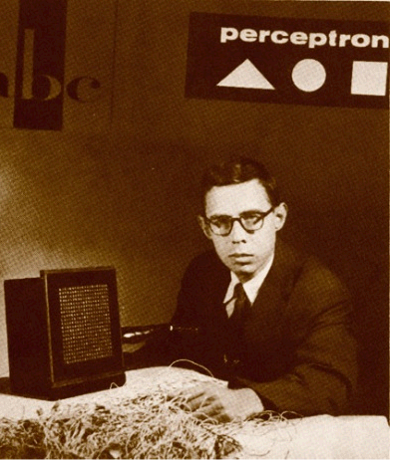
\includegraphics[width=0.5\textwidth]{images/rosenblatt.jpg}
  \caption{Frank Rosenblatt, inventor of the perceptron.}
  \label{fig:rosenblatt}
\end{figure}
\end{minipage}
\hfill
\begin{minipage}{0.45\textwidth}
\begin{quote}
He studied perceptrons, so that the fundamental laws of organization which are common to all information handling systems, machines and men included, may eventually be understood
\end{quote}
- quite a bold statement.
\end{minipage}

We will now briefly introduce ANNs, but we will go into more detail later, in Chapter \ref{ch:neural-networks}.
\subsection{Artificial Neural Networks}
Rosenblatt was influenced in his ANN architecture design by human brains. His implementation is a very, very simplified computational model that uses some aspects of their biological role model.
An ANN consists of \textit{input neuros} ($x_1, x_2, \dots$) that are weighted with corresponding \textit{synaptic weights} ($w_1, w_2, \dots$).
The sum of these weighted inputs is then used to compute the prediction.
The method $f(...)$ is a non-linear function, that we omit for now, which will decide upon the final label
\begin{equation}
  f(\vec{x}) = \left\{\begin{matrix}
    1 \text{ if } \vec{x} \text{ is preferred stimulus}\\
    -1 \text{ otherwise}
  \end{matrix}\right.
\end{equation}

You can see a visualization of such Perceptron in Figure \ref{fig:perceptron}.

\begin{figure}[h]
  \centering
  \begin{tikzpicture}
    \node[draw, circle] (x1) at (0, 0) {$x_1$};
    \node[draw, circle] (x2) at (2, 0) {$x_2$};
    \node[draw, circle] (x3) at (1, -2) {$f\left(\sum_i \vec{\omega}_i \vec{x}_i\righe)$};
    \node (x4) at (1, -4) {$y(\vec{x})$};

    \draw[->] (x1) -- (x3) node [pos=0.66,left,font=\footnotesize] {$\vec{\omega}_1$};
    \draw[->] (x2) -- (x3) node [pos=0.66,right,font=\footnotesize] {$\vec{\omega}_2$};
    \draw[->] (x3) -- (x4);
  \end{tikzpicture}
  \caption{Visualization of a Perceptron.}
  \label{fig:perceptron}
\end{figure}
This is pretty abstract now, but apart from the non-linear function $f(...)$, this is exactly what we saw in the previous chapter.

When Rosenblatt implemented his Perceptron it required a full room of hardware, with massive mechanical relays and giant memory rigs.
Nowadays, we can run the perceptron algorithm on a microcontroller, or even on a small chip that is capable of matrix-vector multiplication.
The original Perceptron algorithm was used to classify handwritten text, we will use exactly the same use case to showcase the algorithm.

\section{The Perceptron Learning Algorithm}
Now we will look deeper into the Perceptron algorithm.
The goal is to perform binary classification of multivariate data points $\vec{x} \in \mathbb{R}^d$.

The input for the algorithm are $N$ tuples of data points $\vec{x}_i$ and their corresponding class labels $y_i$, where $y_i \in \left\{-1, 1\right\}$, such that
\begin{align}
  y_n = \left\{\begin{matrix}
    1 \text{ if } \vec{x}_n \text{ belongs to class }\
    -1 \text{ if } \vec{x}_n \text{ does not belong to class }
  \end{matrix}\right.
\end{align}
additionally the algorithm receives a parameter called \textit{learning rate} $\eta$, we will define this in a second.

The output of the algorithm is a vector of weights $\vec{\omega}$ and a bias $\beta$ that define the linear classifier
\begin{align}
  \vec{\omega}^T \vec{x} + \beta = \left\{\begin{matrix}
    \geq 0 \text{ if } y_n = +1\\
    < 0 \text{ if } y_n = -1
  \end{matrix}\right.
\end{align}
Recall the optimization note in the NCC lecture, where we learned that we can also write $\beta$ into $\vec{\omega}$ by adding a constant dimension to $\vec{x}$
\begin{equation}
  \vec{\hat{\omega}} = \left[\beta,\vec{\omega}\right]^T, \vec{\hat{x}} = \left[1, \vec{x}\right]^T
\end{equation}

\ssection{The Perceptron Error Function}
This is a reformulation of the perceptron loss function from Table \ref{tab:error_functions}
\begin{equation}
  \Epsilon(\vec{x}, y, \vec{\omega}) = \max\left(0, -y \vec{\omega}^T \vec{x}\right) = -\sum_{m \in \mathcal{M}} \vec{\omega}^T \vec{x}_m y_m
\end{equation}
where $\mathcal{M}$ is the set of all misclassified data points.

\subsection{Classification Error as Function of weights}
You can see a plot of this error function in Figure \ref{fig:perceptron_error_function}. On the left side we have all correct classified labels, on the right the misclassified ones.

Now, let's look at a real 2D example data set. On the right side you can see a plot for the error, if we project our $\vec{\omega}$ vector onto any point in our coordinate system on the left side.

So each point on the right grid represents a potential $\vec{\omega}$ vector. The color of the point represents the error of this $\vec{\omega}$ vector.
To find the best value for $\vec{\omega}$ we must find the minimum of this error function. But usually we can't just simply create this plot, nor can we try out every possible value for $\vec{\omega}$ in finite time.
So in general, what we do in ML is, to randomly initialize $\vec{\omega}$ and evaluate our error function. But instead of evaluating the regular error function, we evaluate it's gradient.
This gives us the steepness of the error function in $\vec{\omega}$. To minimize the error through $\vec{\omega}$ we then adjust $\vec{\omega}$ in the opposite direction of the gradient.
This works, because the gradient of the error function points into the direction of the biggest error.
This process is called \textit{Gradient Descent (GD)} and is a very popular optimization technique in ML.
\section{Gradient Descent}
\label{sec:gradient_descent}
Gradient Descent is, as we just saw, an algorithm that can optimize a function $f(\vec{x}, \vec{\omega})$ by iteratively adjusting the parameters $\vec{\omega}$ in the opposite direction of the gradient of $f$. Hence we can use GD to minimize the error function of the Perceptron algorithm.

We randomly initialize $\vec{\omega}$ and then iteratively update it by subtracting the gradient of the error function $\Epsilon(\vec{x}, y, \vec{\omega})$.
And this is how GD works in detail
We have an old value for $\vec{\omega}$, $\vec{\omega}^{\text{old}}$, e.g. randomly initialized, compute the gradient of the error function using $\vec{\omega}^{\text{old}}$ by summing over all training samples that is scaled by $\eta$, the learning rate, to compute
\begin{equation}
  \vec{\omega}^{\text{new}} = \vec{\omega}^{\text{old}} - \eta \sum_{i=1}^{X} \nabla_{\vec{\omega}} \Epsilon(\vec{x}, y, \vec{\omega})
\end{equation}
Here you can see why this algorithm is called GD, we subtract the current gradient from our current weights. The learning rate $\eta$ determines how fast we descent.
The resulting $\vec{\omega}^{\text{new}}$ will be the new adjusted weights from our model. We can now repeat this process until we reach a certain threshold in the error, or until we reach a certain number of iterations.

\subsection{Stochastic Gradient Descent}
\subsection{Mini-Batch Gradient Descent}

\section{Perceptron Training}
\section{Problems with the Perceptron Algorithm}
\section{Application Example: Handwritten Digits}
\section{Derivation of the Perceptron Error Function}

\section{Combining multiple Perceptrons}
\label{sec:combining_perceptrons}

\subsection{One-vs-All}
\subsection{One-vs-One}

\subsection{Application Example: Handwritten Digits (multi-class)}

\framedtext{\color{red}{TODO:}}



\chapter{Decision Trees}
\label{ch:decision-trees}

Decision trees are another group of supervised learning algorithms.
They are used for both classification and regression problems.
Decision trees are easy to understand and interpret, and they are
very useful for exploratory data analysis. 
They are also the basis for more sophisticated methods we will introduce at the end of this chapter.
Similar to the KNN algorithm, decision trees are also non-parametric methods, which use the data 
as the model itself.
But different to the KNN algorithm, decision trees are non linear algorithms in the classical sense.
We will also see that there is a relation of decision trees to linear models.

\section{Classification Trees}
In this chapter and in the book we will only look into classification trees.
The regression trees are very similar, but we will not discuss them here.

Before we begin, we must introduce important concepts that construct decision trees.

A \textit{tree} is a hierarchical structure consisting of \textit{nodes} and \textit{edges}.
Nodes are connected by edges, and the edges are directed from the \textit{parent} node to the \textit{child} node.
For simplicity, we will only consider binary trees, where each node has at most two children.
Nodes without children are called \textit{leaves} or \textit{terminal nodes}, and nodes with children are called \textit{internal nodes} or \textit{decision nodes}.
The top node of a tree is called the \textit{root node}.
You can see a very simple example of a tree in Figure \ref{fig:tree_simple}.
\begin{figure}[ht]
  \centering
  \begin{tikzpicture}[sibling distance=10em,
    every node/.style = {shape=rectangle, rounded corners,
      draw, align=center,
      top color=white, bottom color=blue!20}]]
    \node {Root Node}
      child { node {Child \#1} }
      child { node {Child \#2} };
  \end{tikzpicture}
  \caption{Simple decision tree.}
  \label{fig:tree_simple}
\end{figure}

\subsection{Motivational Examples}
Let us consider a simple example to motivate the idea of decision trees.
Imagine you want to plan a dinner party. And you need to decide whether you host
the party inside or outside. You have a lot of friends, and you want to invite as many as possible.

You come up with the decision tree shown in Figure \ref{fig:tree_dinner}.
\begin{figure}[ht]
  \centering
  \begin{tikzpicture}[sibling distance=10em,
    every node/.style = {shape=rectangle, rounded corners,
      draw, align=center,
      top color=white, bottom color=blue!20}]]
    \node {Raining?}
      child { node {Inside} }
      child { node {Cold?}
        child { node {Inside} }
        child { node {Outside} }
      };
  \end{tikzpicture}
  \caption{Decision tree for planning a dinner party. Left nodes answer the short questions with \textit{yes}, right nodes with \textit{no}.}
  \label{fig:tree_dinner}
\end{figure}
From looking at this tree we can make two major observations.
First, the tree is a sequence of binary questions that we can answer with \textit{yes} or \textit{no}.
Second, the tree is a sequence of decisions that lead to a final decision.
We can also see that the tree is a sequence of \textit{if-then-else} statements.\\
If it is raining, we host the party inside, else we ask the next question.\newline
If it is cold, we host the party inside, else we host the party outside.

This sounds simple to implement, but how do we come up with these questions?
\subsection{Building a Decision Tree}
In a very simplistic way to build a decision tree, we need to follow the following three steps
\begin{enumerate}
  \item Split the data in "the best way possible"
  \item continue this process with every new left and right side, until satisfied
  \item create leaf nodes for final splits, assign label of majority of remaining samples to the leaf node
\end{enumerate}
But what does "the best way possible" mean? We will try to understand this based on the following example.
\subsection{Linearly Seperable Data}
Given the following linear seperable data $X$ and accomodating labels $y$, find the correct split to perform binary classification
\begin{align}
  X = \begin{bmatrix}
    0.3\\0.37
  \end{bmatrix},
  \begin{bmatrix}
    0\\1
  \end{bmatrix}
\end{align}
The solution to this is rather obvious
\begin{align}
f(x) = 
\left\{
\begin{matrix}
0 \text{ if } x \leq 0.3\\
1 \text{ if } x > 0.3
\end{matrix}
\right.
\end{align}
or as a decision tree (Figure \ref{fig:tree_linear_1}).
\begin{figure}[ht]
  \centering
  \begin{tikzpicture}[sibling distance=10em,
    every node/.style = {shape=rectangle, rounded corners,
      draw, align=center,
      top color=white, bottom color=blue!20}]]
    \node {x $\leq$ 0.3}
      child { node {0} }
      child { node {1} };
  \end{tikzpicture}
  \caption{Decision tree for very simplistic linear seperable data.}
  \label{fig:tree_linear_1}
\end{figure}

We can break down the decision process for the numerical value $x$ and selected threshold $0.3$ into two steps
\begin{enumerate}
  \item Select the best possible feature
  \subitem In this case, we only have one feature, so we do not need to select one
  \item Find the value in $x$ that separates the classes best
  \subitem In this case, we can see that the value $0.3$ is the only value available that represents the class $0$ and $0.37$ the only sample of class $1$
\end{enumerate}

With increasing amount of data points this process becomes increasingly hard to perform, manually.

Consider the following data
\begin{align}
X = \begin{pmatrix}
0.35, 0.6, 0.67, 0.8
\end{pmatrix}^T\\
y = \begin{pmatrix}
0, 0, 1, 1
\end{pmatrix}^T
\end{align}
The optimal solution is still very obvious
\begin{align}
f(x) = 
\left\{
\begin{matrix}
0 \text{ if } x \leq 0.6\\
1 \text{ if } x > 0.6
\end{matrix}
\right.
\end{align}
or as tree
\begin{figure}[ht]
  \centering
  \begin{tikzpicture}[sibling distance=10em,
    every node/.style = {shape=rectangle, rounded corners,
      draw, align=center,
      top color=white, bottom color=blue!20}]]
    \node {x $\leq$ 0.6}
      child { node {0} }
      child { node {1} };
  \end{tikzpicture}
  \caption{Decision tree for more linear seperable data.}
  \label{fig:tree_linear_2}
\end{figure}

\subsection{Non-Linearly Seperable Data}
Given the following non-linear seperable data $X$ and accomodating labels $y$, find the correct split to perform binary classification
\begin{align}
X = \begin{pmatrix}
0.3, 0.1, 0.21, 0.35, 0.6, 0.67, 0.8, 0.786, 0.97
\end{pmatrix}^T\\
y = \begin{pmatrix}
0, 0, 1, 0, 1, 1, 0, 1, 0
\end{pmatrix}^T
\end{align}
In this example we can not simply split the data by briefly looking at it and visually recognize
the seperation. We need to find a way to split the data in a way that we can seperate the classes
as good as possible. For this we need to understand what a split actually is, how we can evaluate
the quality of a split and how we can find the best split. Additionally, when we have
multivariate data, we need to understand how we can select the best feature to split on.

\section{Information Gain}
The information gain $\text{Gain}$ tells us how much information we gain over $x$ while looking at $y$.
This metric can be used to evaluate the quality of a split. It measures the reduction
of an impurity metric in a splitted data set.
The information gain is defined as
\begin{align}
  \text{Gain}(S, V) = I(S) - \sum_{S_v\in V} \frac{|S_v|}{|S|}I(S_v)
\end{align}
with $V$ a set of splits out of $S$.  
For two splits
\begin{align}
\text{Gain}(S, V) = I(S) - \left(\frac{|S_1|}{|S|}I(S_1)+\frac{|S_2|}{|S|}I(S_2)\right)
\end{align}

\section{Impurity Metrics}
The impurity metric $I$ is a metric that measures the impurity of a data set.
The following metrics are calculated at the node level. The lower their value, the purer the observed data.
\subsection{Entropy}
The entropy is a measure of the uncertainty of a random variable and ranges from $0$ to $1$. It is defined as
\begin{align}
  I(S) = -\sum_{i=1}^n p_i \log_2 p_i
\end{align}
with $p_i$ the probability randomly selecting a sample of class $i$ out of the $k$ classes in $S$.

In Python, we can calculate the entropy as follows
\begin{lstlisting}[language=Python]
def entropy(s):
  counts = np.bincount(np.array(s, dtype=np.int64))
  percentages = counts / len(s)
  return -np.sum([
    pct*np.log2(pct)
    for pct in percentages
    if pct > 0
  ])
\end{lstlisting}

\subsection{Gini Impurity}
The Gini impurity is a measure of the probability of a random sample being classified incorrectly if it was randomly labeled according to the distribution of labels in the subset. Hence it combines the probability of randomly selecting an item $i$
\begin{align}
  p_i = \frac{|S_i|}{|S|}
\end{align}
with the probability of misclassifying an item $i$
\begin{align}
  \sum_{j\neq i} p_j = 1 - p_i = \frac{|S| - |S_i|}{|S|}
\end{align}
Thereby, the Gini impurity is defined as
\begin{align}
  I(S) = \sum_{i=1}^cp_i (1 - p_i) = \sum_{i=1}^c (p_i - p_i^2)\\
  = \underbrace{\sum_{i=1}^c p_i}_{:= 1} + \sum_{i=1}^c p_i^2 = 1 - \sum_{i=1}^c p_i^2
\end{align}

In Python, we can calculate the Gini impurity as follows
\begin{lstlisting}[language=Python]
def gini_impurity(s):
    counts = np.bincount(np.array(s, dtype=int))
    percentages = counts / len(s)
    return 1 - (percentages**2).sum()
\end{lstlisting}

Both metrics are very similar, but the Gini impurity is slightly faster to compute due to the lack of logarithm.
They also share some properties. A low impurity measure translates to a low likelihood of misclassification. A high value translates to a high likelihood of misclassification.

\subsection{Prediction Error}
Another metric is the prediction error. It is defined as
\begin{align}
  I(S) = 1 - \max_i p_i
\end{align}
and is essentially the inverse of the maximum probability of correctly classifying a sample for any given class in $S$.\\
This metric is not as useful as the other two to construct decision trees, but it is useful to evaluate the quality of a tree to optimize it.
One way of optimizing decision trees is to reduce their amount of decision nodes.
This can be done by pruning the tree. Pruning is the process of removing decision nodes from a tree.
We will discuss this in more detail shortly.

Implemented in Python, the prediction error looks like this
\begin{lstlisting}[language=Python]
def prediction_error(s):
    counts = np.bincount(np.array(s, dtype=int))
    percentages = counts / len(s)
    return 1 - np.max(percentages)
\end{lstlisting}

\subsection{Comparison of Impurity Metrics}
For comparison we will compute the impurity meytics for 101 different combinations of binary labels for 100 samples.

In Python, we could do something like this
\begin{lstlisting}[language=Python]
g = list(); e = list(); e2 = list(); err = list(); bins = list()
for i in range(101):
    values = [0] * (100 - i) + [1] * i
    g.append(gini_impurity(values))
    e.append(entropy(values))
    e2.append(np.array(entropy(values))/2.)
    err.append(error(values))
    bins.append(values)
\end{lstlisting}
and we can visualize these results with the following code
\begin{lstlisting}[language=Python]
import matplotlib.pyplot as plt

def draw_bins(bins, alpha=0.5):
  for idx, val in enumerate(bins):
    unique, counts = np.unique(val, return_counts=True)
    if idx == 0:
      counts = np.array([len(val), 0])
    elif idx == len(bins) - 1:
      counts = np.array([0, len(val)])
    plt.bar(
      [idx,idx+0.5],
      height=counts/len(val),
      width=0.5,
      color=['b', 'g'],
      label=['class 0', 'class 1'],
      alpha=alpha
    )
\end{lstlisting}
\begin{figure}[ht]
  \begin{minipage}{0.5\textwidth}
    \centering
    \includesvg[width=.95\textwidth]{images/DT_comparison_1.svg}
    \caption{Impurity metrics for 101 different combinations of binary labels for 100 samples.}
    \label{fig:impurity_metrics}
  \end{minipage}
  \begin{minipage}{0.5\textwidth}
    \centering
    \includesvg[width=.95\textwidth]{images/DT_comparison_2.svg}
    \caption{Rescaled impurity metrics for 101 different combinations of binary labels for 100 samples.}
    \label{fig:impurity_metrics_zoomed}
  \end{minipage}
\end{figure}
The entropy ranges from $0$ pure to $1$ impure, whereas the Gini impurity ranges from $0$ pure to $0.5$ impure as you can see in Figure \ref{fig:impurity_metrics}.
To visualize the relationship between the two metrics, we can rescale the entropy by dividing it by $0.5$. 
This allows us to see that the Gini impurity lies between the Entropy and the prediction error and is not a differently scaled Entropy (see Figure \ref{impurity_metrics_zoomed}).

Depending on the chosen metric the resulting trees can vary. Sometimes this makes a small impact,
sometimes a bigger one. Overall, Entropy and Gini impurity are implemented in many algorithms.
CART (Classification and Regression Trees) uses the Gini impurity, whereas ID3 (Iterative Dichotomiser 3) uses the Entropy.

Most of these implementations like C5 are highly optimized using methods like \textit{boosting}
 that improve the structure of the trees by selecting better splits.

\section{Disadvantages of Decision Trees}
The biggest and main disadvantage of decision trees is that deep trees are prone to overfitting the training data. On the other hand, shallow trees increase the risk of biased predictions.

One solution for this is called \textit{Random Forrest}. It is an ensemble method that combines multiple decision trees to reduce the risk of overfitting without sacrificing bias.
Random Forrests are more robust and generally better solvers than single decision trees.


\section{Decision Trees in scikit-learn}
You can find an implementation based on NumPy in the accomodating Jupyter notebook to this chapter.
In this section we will look at the implementation of decision trees in scikit-learn and apply it to the Iris data set.

The decision tree classifier is implemented in the \texttt{DecisionTreeClassifier} class.
It is, as it name suggests, the implementation of the classification variant of Decision Trees and has the following parameters
\begin{itemize}
  \item \texttt{criterion}: The impurity metric to use. Either \texttt{gini} or \texttt{entropy}.
  \item \texttt{max\_depth}: The maximum depth of the tree. If \texttt{None}, the tree is grown until all leaves are pure.
  \item \texttt{min\_samples\_split}: The minimum number of samples required to split an internal node.
  \item \texttt{min\_samples\_leaf}: The minimum number of samples required to be at a leaf node.
  \item \texttt{min\_impurity\_decrease}: A node will be split if this split induces a decrease of the impurity greater than or equal to this value.
  \item \texttt{class\_weight}: Weights associated with classes in the form \texttt{\{class\_label: weight\}}.
  \item \texttt{random\_state}: The seed of the pseudo random number generator to use when shuffling the data.
  \item \texttt{max\_features}: The number of features to consider when looking for the best split.
\end{itemize}

You can see an example usage of the decision tree classifier in Listing \ref{lst:dtc}.
\begin{lstlisting}[language=Python, caption={Example usage of the decision tree classifier.}, label={lst:dtc}]
from sklearn.datasets import load_iris
from sklearn.tree import DecisionTreeClassifier
from sklearn.model_selection import train_test_split

# load data
iris = load_iris()
X = iris.data

# split into train and test set
X_train, X_test, y_train, y_test = train_test_split(
  X, iris.target, test_size=0.2, random_state=42
)

dtc = DecisionTreeClassifier()
dtc.fit(X_train, y_train)

print('Accuracy:', dtc.score(X_test, y_test))
\end{lstlisting}
As discussed in the HPO chapter (Chapter \ref{ch:hpo}), we can use for instance the \texttt{GridSearchCV} class to find the best parameters for our model.
You can see an example usage of this in Listing \ref{lst:dtc_gridsearch}.
\begin{lstlisting}[language=Python, caption={Example usage of the decision tree classifier with grid search.}, label={lst:dtc_gridsearch}]
from sklearn.datasets import load_iris
from sklearn.tree import DecisionTreeClassifier
from sklearn.model_selection import train_test_split, GridSearchCV

# load data
iris = load_iris()
X = iris.data

# split into train and test set
X_train, X_test, y_train, y_test = train_test_split(
  X, iris.target, test_size=0.2, random_state=42
)

dtc = DecisionTreeClassifier()

params = {
  'criterion': ['gini', 'entropy'],
  'max_depth': [None, 2, 4, 6, 8, 10],
  'min_samples_split': [2, 4, 6, 8, 10],
  'min_samples_leaf': [1, 2, 3, 4, 5],
  'min_impurity_decrease': [0.0, 0.1, 0.2, 0.3, 0.4, 0.5],
  'class_weight': [None, 'balanced'],
  'random_state': [42],
  'max_features': [None, 'auto', 'sqrt', 'log2']
}

grid = GridSearchCV(dtc, params, cv=5, n_jobs=-1)
grid.fit(X_train, y_train)

print('Best score:', grid.best_score_)
print('Best params:', grid.best_params_)
print('Accuracy:', grid.score(X_test, y_test))
\end{lstlisting}



\framedtext{\color{red}{TODO:}} Finalize example



\chapter{Regression}
\label{ch:regression}
\framedtext{\color{red}{TODO:}}

\chapter{Principal Component Analysis (PCA)}
\label{ch:pca}
\framedtext{\color{red}{TODO:}}
\chapter{Linear Discriminant Analysis (LDA)}
\label{ch:lda}
\framedtext{\color{red}{TODO:}}
\chapter{Support Vector Machines (SVM)}
\label{ch:svm}
\framedtext{\color{red}{TODO:}}
\chapter{Naive Bayes}
\label{ch:naive-bayes}
\framedtext{\color{red}{TODO:}}
\chapter{Clustering}
\label{ch:clustering}
\framedtext{\color{red}{TODO:}}

\chapter{Artificial Neural Networks \& Deep Learning}
\label{ch:neural-networks}
\framedtext{\color{red}{TODO:}}
\section{Multilayer Perceptron (MLP)}
\label{sec:mlp}
\framedtext{\color{red}{TODO:}}
\section{Convolutional Neural Networks (CNN)}
\label{sec:cnn}
\framedtext{\color{red}{TODO:}}
\section{Recurrent Neural Networks (RNN)}
\label{sec:rnn}
\framedtext{\color{red}{TODO:}}
\section{Long Short-Term Memory (LSTM)}
\label{sec:lstm}
\framedtext{\color{red}{TODO:}}
\section{Transformers}
\label{sec:transformers}
\framedtext{\color{red}{TODO:}}
\subsection{Attention}
\label{subsec:attention}
\framedtext{\color{red}{TODO:}}
\subsection{Self-Attention}
\label{subsec:self-attention}
\framedtext{\color{red}{TODO:}}
\subsection{Multi-Head Attention}
\label{subsec:multi-head-attention}
\framedtext{\color{red}{TODO:}}
\subsection{BERT}
\label{subsec:bert}
\framedtext{\color{red}{TODO:}}
\subsection{GPT}
\label{subsec:gpt}
\framedtext{\color{red}{TODO:}}



\chapter{Natural Language Processing (NLP)}
\label{ch:nlp}
\framedtext{\color{red}{TODO:}}
\chapter{Computer Vision}
\label{ch:computer-vision}
\framedtext{\color{red}{TODO:}}
\chapter{Generative Artificial Intelligence}
\label{ch:generative-ai}
\framedtext{\color{red}{TODO:}}
\chapter{Reinforcement Learning}
\label{ch:reinforcement-learning}
\framedtext{\color{red}{TODO:}}

\newpage
{
  \pagenumbering{roman}
  \setcounter{page}{1}
  \appendix
\chapter{Visualizations}

\begin{figure}[h]
  \centering
  \begin{minipage}{.45\textwidth}
  \centering
    \includesvg[width=.95\textwidth]{images/NCC_frame_0.svg}
    %\caption{Both means start at the origin}
    \label{fig:ncc_streaming_0}
  \end{minipage}
  \hfill
  \begin{minipage}{.45\textwidth}
  \centering
    \includesvg[width=.95\textwidth]{images/NCC_frame_1.svg}
    %\caption{The mean of the blue class (red) is updated.}
    \label{fig:ncc_streaming_1}
  \end{minipage}\\
  \begin{minipage}{.45\textwidth}
  \centering
    \includesvg[width=.95\textwidth]{images/NCC_frame_2.svg}
    %\caption{After adding the second blue sample, the mean is updated again to its final position}
    \label{fig:ncc_streaming_2}
  \end{minipage}
  \hfill
  \begin{minipage}{.45\textwidth}
  \centering
    \includesvg[width=.95\textwidth]{images/NCC_frame_3.svg}
    %\caption{The first orange sample is added to the mean of the orange class (green)}
    \label{fig:ncc_streaming_3}
  \end{minipage}\\
  \begin{minipage}{.45\textwidth}
  \centering
    \includesvg[width=.95\textwidth]{images/NCC_frame_4.svg}
    %\caption{The last orange sample is added to the mean of the orange class (green) and the mean is updated to its final position}
    \label{fig:ncc_streaming_4}
  \end{minipage}
  \caption{Nearest Centroid Classifier (NCC) with streaming updates for 4 samples of two classes. The blue class is represented by the red mean and the orange class by the green mean. The blue samples are represented by blue dots and the orange samples by orange dots. The mean of the blue class is updated after adding the first (Figure \ref{fig:ncc_streaming_1}) and second blue sample (Figure \ref{fig:ncc_streaming_2}). The mean of the orange class is updated after adding the first (Figure \ref{fig:ncc_streaming_3}) and last orange sample (Figure \ref{fig:ncc_streaming_4}).}
  \label{fig:ncc_batched_streaming}
\end{figure}



  \addcontentsline{toc}{chapter}{Bibliography}
  \bibliographystyle{/opt/ieeetran/IEEEtran/bibtex/IEEEtran}
  \bibliography{/opt/ieeetran/IEEEtran/bibtex/IEEEabrv,refs}
}
\end{document}
